\documentclass[12pt]{article}
\usepackage[utf8]{inputenc}
\usepackage[left=35mm, right=35mm, top=35mm, bottom=15mm, includefoot]{geometry}
\usepackage[sorting=none]{biblatex}
\usepackage{graphicx}
\usepackage{amsmath}
\usepackage{times}
\usepackage[numbib]{tocbibind}  
\usepackage[center]{caption}
\usepackage{adjustbox}
\usepackage{afterpage}
\usepackage{indentfirst}
\usepackage{listings}
\newtheorem{theorem}{Theorem}[section]
\addbibresource{bib.bib}
\graphicspath{ {./figures/} }

\title{Comparison of network complexity meausres}
\author{Yipei Zhao}

\date{October 2021}
\begin{document}
\begin{titlepage}
    \begin{center}
        \vspace*{1cm}
 
        {\Huge Comparison of network complexity meausres}
 
        \vspace{0.5cm}
         
             
        \vspace{1.5cm}
 
        \textbf{Yipei Zhao}\\
        Student number: 170145594\\
        A thesis presented for the degree of\\
        Master of Science Data Analytics\\
        {\large Supervised by Jens Christian Cluassen}\\
        October 2021
 
        \vfill
             

    \end{center}
 \end{titlepage}

\tableofcontents
\pagebreak
\renewcommand{\familydefault}{}
\section{Introduction}
\par
In modern world, there are many fields where a network can be investigated and studied. For example, electric cables in a region would form a large network.\cite{5275353} Also, analysing social networks and use their unique properties to drop promotion precisely would help firms to increase profits.\cite{stefko2011virtual} In addition, food webs can be considered as networks and they have been
studied for many years.\cite{dunne2002food} There are many aspects of a network, but it is vital to ask: what is the complexity of a network? How a network to be designed as complex/simple? The goal of this project is to summarise and compare different complexity measures, including implementations and applications on different real networks.
\par
In this project, we want to be specific on transport networks. A transport network transfer either passengers or goods with the flow, from initial location to their destination. To apply complextiy of transport networks, the designers of the network have to think about this: how do I modify the complexity of the network and what change will it bring to the network? Transport networks is different to common networks in real world, but before investigate the uniqueness of transport network, it is vital to study network science as a whole.\\
\begin{figure}[!h]
    \centering
    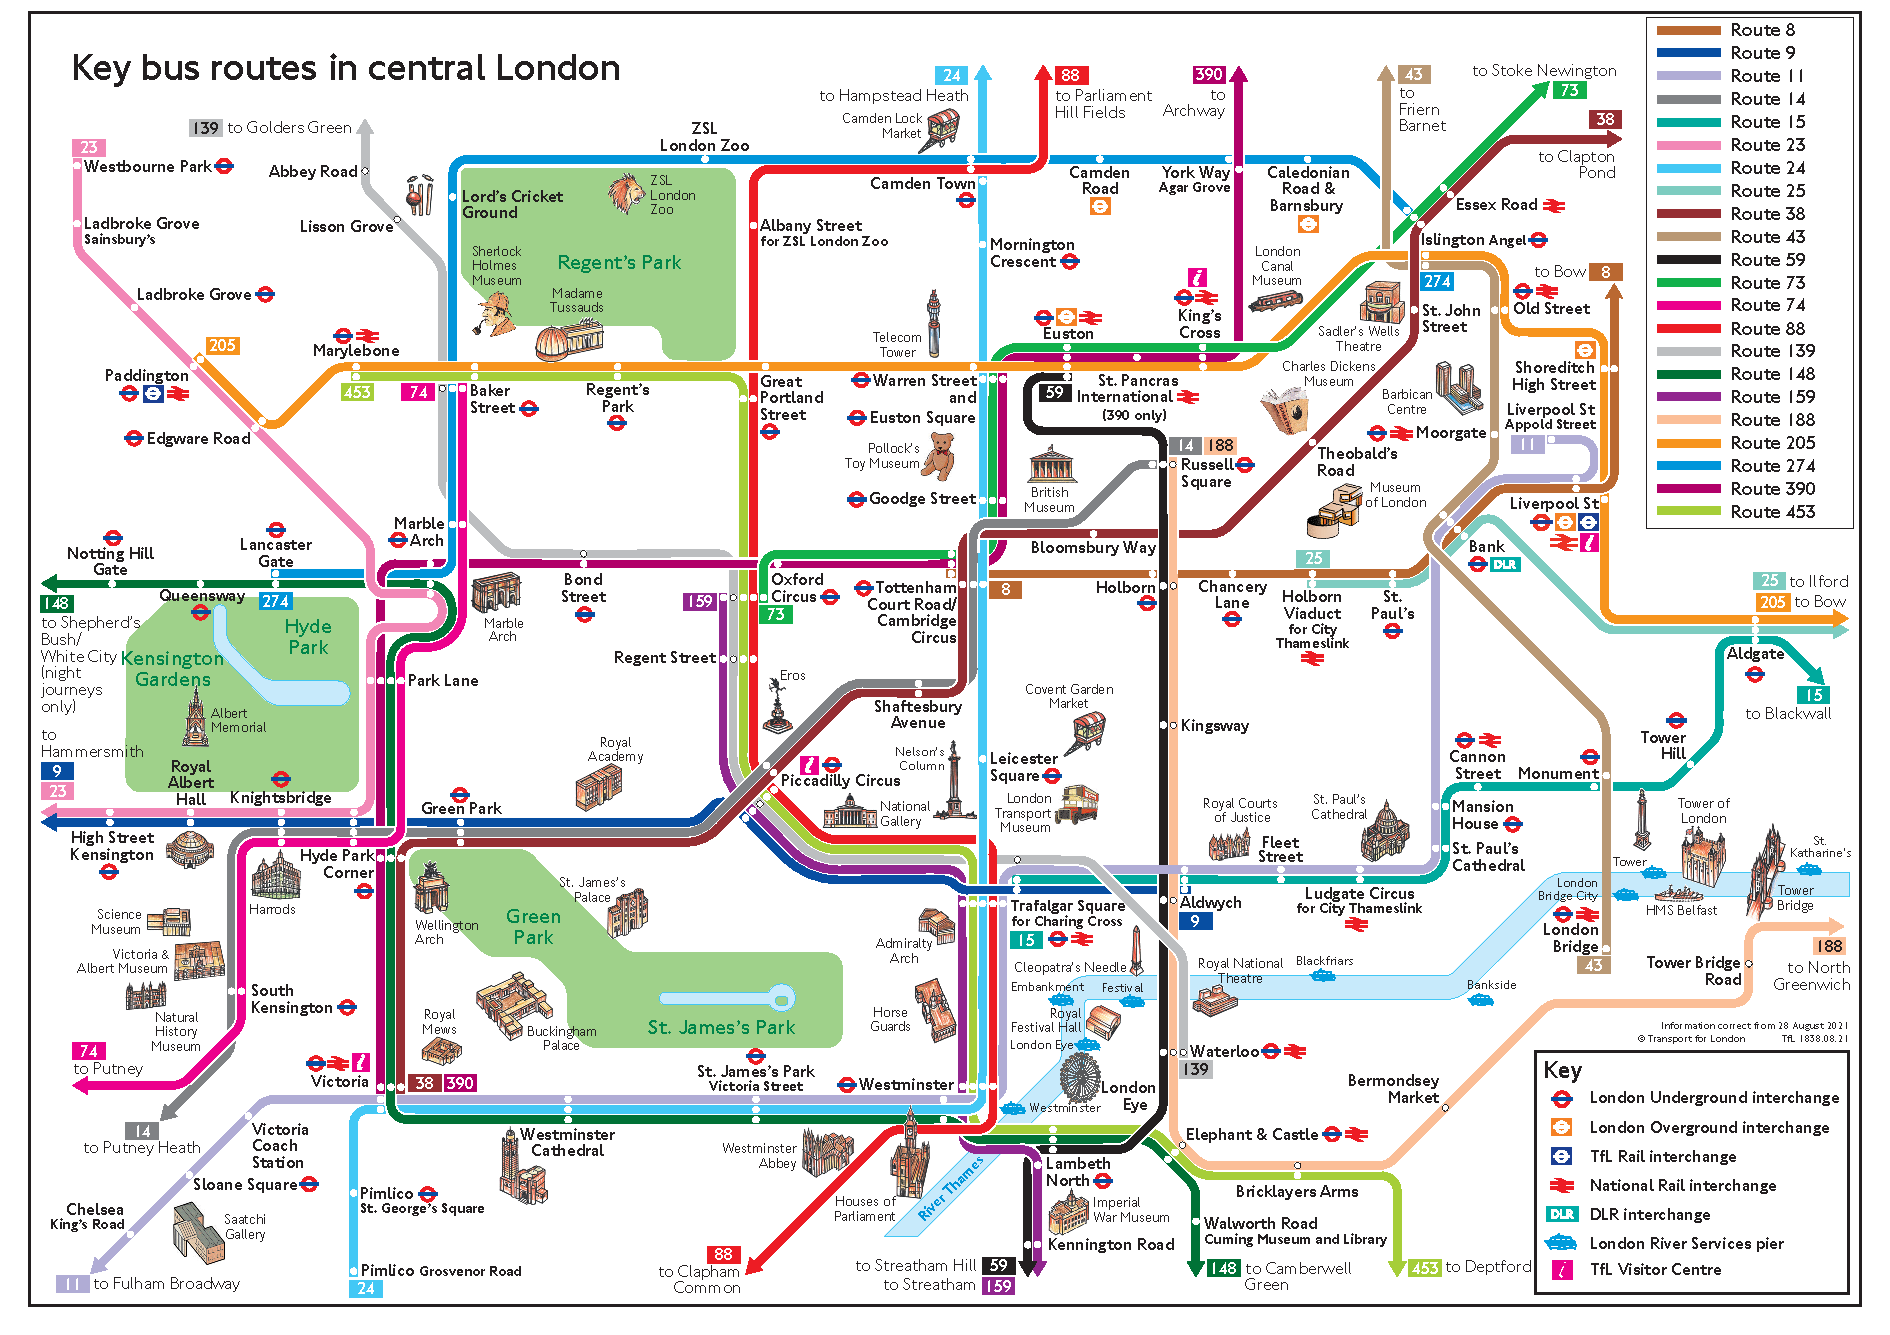
\includegraphics[width=\textwidth]{key-bus-routes-in-central-london.pdf}
    \caption{Key routes in central London.\cite{london_bus}}
\end{figure}

\subsection{Graph theory}
Firstly, what does network scientists study? A network contains $n$ nodes/vertices and $m$ edges/links, nodes can be connected using edges. Allowing construcion of assets. In a transport network, a node can be consdiered as a stop on the road and edges are the roads/path connecting stops.
\begin{center}
    "we view network science as the study of the collection,
    management, analysis, interpretation, and presentation of relational data" \cite{brandes_robins_mccranie_wasserman_2013}
\end{center}

\subsubsection{Graph}
\label{graph}
To stay simple, all networks in this project have the following properties:
\begin{itemize}
    \item Undirected. Edges are not allowed to have direction. If the graph is originally directed, it will be turned into an undirected graph.
    \item Unweighted. All the edges are fairly recognized and no weights are assgined.
    \item No multi-edges. There will be at most one edge between two nodes.
    \item No self-links. Nodes are not allowed to connect to themselves. 
\end{itemize}
\begin{theorem}{(Graph/network)}
    A graph or network $G$ can be represented by three sets. A node set $V:\{V_1,V_2,V_3...V_n\}$ and an edge set $E:\{E_1,E_2,E_3...E_m\}$ and a function set $\iota$ such that $E\rightarrow V_\alpha\times V_\beta$ implies there is a connection between node $V_\alpha$ and node $V_\beta$.
\end{theorem}
\par
In non-mathematicial words, a network or a graph is a collection of nodes and edges, each node can connect to other nodes via edges.The border between the term network and graph is very ambiguous, and network scientists use them interchangeably. There are many different type of graphs. A path graph contains $n$ nodes and all nodes are connected in a consequence, or a clique which all nodes are connected to others. Since a clique connects all its nodes, leads to a number of $n(n-1)/2$ edges in total.
\begin{figure}[!h]
    \centering
    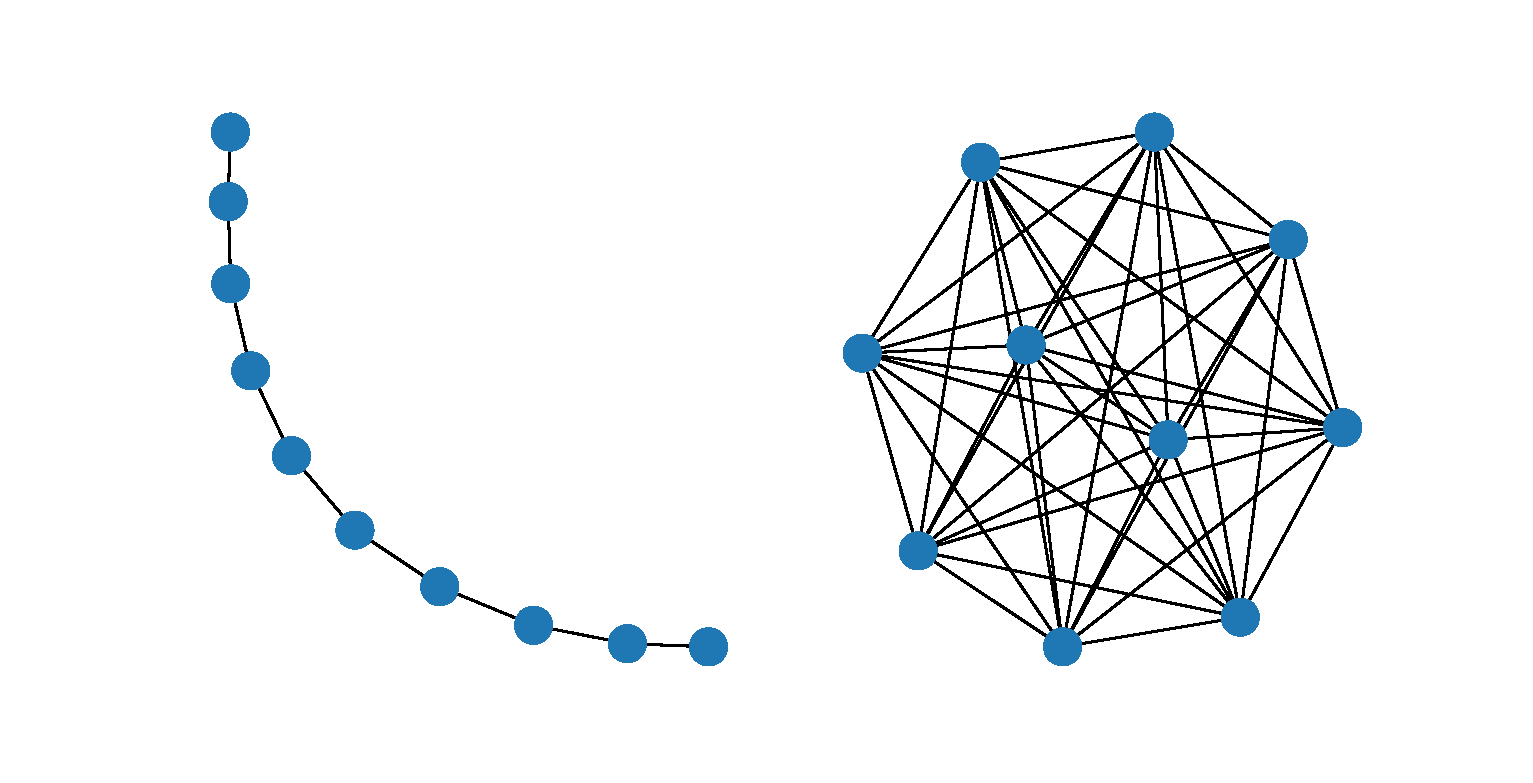
\includegraphics[width=0.8\textwidth]{path_clique.eps}
    \caption{From left to right: A path with 10 nodes($n=10$) and 9 edges($m=9$); a clique with 10 nodes and 45 edges($m=45$).}
\end{figure}
\begin{theorem}{(Subgraph)}
    A subgraph $G'$ is a slice of a graph $G$, such that $V' \epsilon V$, $E' \epsilon E$ and $\iota'$ matches two nodes belongs to $V'$, i.e. $E'\rightarrow V'_\alpha\times V'_\beta $. All the edges must have their starting and ending points within the subgraph.
\end{theorem}
\begin{theorem}{(Neighbours)}
    If node $i$ is connected to node $j$, node $i$ is a neighbour of node $j$, vice versa. If node $i$ is connected to node $j,k,l$, the node set $\{j,k,l\}$ is said to be the neighbourhood of node $i.$
\end{theorem}
\begin{theorem}{(Distance)}
    Distance $d_{i,j}$ in a undirected, unweighted graph is the minimum number of edges required to connect node $i$ and $j$. Average distance $\langle d\rangle$ is defined as $\langle d \rangle = \frac{2}{n(n-1)}\sum_{i,j}d_{i,j}$.
\end{theorem}
\begin{figure}[!h]
    \centering
    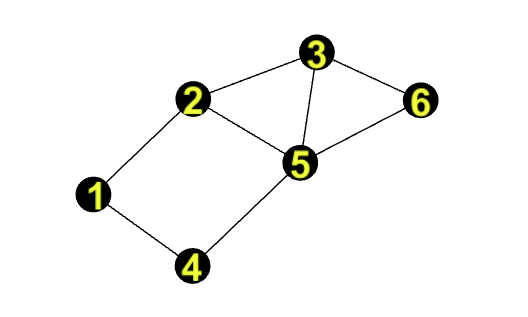
\includegraphics[width=0.8\textwidth]{simplenetwork.png}
    \caption{A simple network with 6 nodes and 8 edges.}
    \label{fig:simple_network}
\end{figure}
\par
Refereing to figure \ref{fig:simple_network}, distance between node 1 and 6 is 3, denoted by $d_{1,6}=d_{6,1}=3$. Distance between node $i$ and node $j$ is equal to node $j$ to node $i$: $d_{i,j}=d_{j,i}$. The average distance of the network is 1.53.

\par
A node $i$ has degree $k_i$ if it has $k$ edges connected to other nodes. For figure \ref{fig:simple_network}, we have $k_1=2,k_2=3,k_3=3,k_4=2,k_5=4,k_6=2$. Thus, the total number of edges $L$ in a network can be calculated:
\begin{equation}
    L = \frac{1}{2}\sum^{i}_{i=0}{k_i}
    \label{eqn:numberoflinks}
\end{equation}
Using equation \ref{eqn:numberoflinks}, we can calculate the total number of links for figure \ref{fig:simple_network} is equal to:\\
\begin{equation}
    L =\frac{1}{2}(2+3+3+2+4+2)=8
\end{equation}
An important parameter of a network is generated using degrees, which is average degree of a network:
\begin{equation}
    \bar{k}=\frac{1}{N} \sum^{i}_{i=0}{k_i}
    \label{eqn:avg_degree}
\end{equation}
or, simply:
\begin{equation}
    \bar{k}=\frac{2L}{N}
    \label{eqn:avg_degree_1}
\end{equation}
Applying formula \ref{eqn:avg_degree} to figure \ref{fig:simple_network}, the average degree is:
\begin{equation}
    \bar{k} = \frac{1}{6}(2+3+3+2+4+2)=\frac{8}{3}
\end{equation}
or equivalently, using formula \ref{eqn:avg_degree_1}:
\begin{equation}
    \bar{k} = \frac{1}{6}(8*2)=\frac{8}{3}
\end{equation}
\begin{theorem}{(Clustering coefficient)}
    Clustering coefficient $C_i$ illustrates the proportion of edges exists between a node $i$'s neighbours. For a given node $i$ with degree $k$, the clustering coefficient is defined as:\\
    $C_i=\frac{2L_i}{k_i(k_i-1)}$\\
    where $L_i$ represents the number of links exists between node $i$'s neighbours.
\end{theorem}
\par 
In figure \ref{fig:simple_network}, node 2 and node 4 are node 1's neighbours. There are no edges between node 2 and node 4, so $C_1 = 0$. On the otherhand, node 3 has neighbours 2,5 and 6. There are 2 edges between node 2,5 and 6, $C_i=\frac{2*2}{3*2}=\frac{2}{3}$. Average clustering tends to suggest the average connectivity of the network.

\begin{theorem}{(Laplacian Matrix)}
    A Laplacian matrix is defined as:
    \begin{equation}
        L_{i,j} = \begin{cases}
            k_{i}& \text{if i=j}\\
            -1 & \text{if an edge exists between node i and j, and i is not equal to j}\\
            0 & \text{otherwise}
        \end{cases}
    \end{equation}
\end{theorem}
\par
Diagonal elements $L_{i,i}$ suggests the degree of node $i$.A non-zero non-diagonal element $L_{i,j}$ implies a connected edge between node $i$ and $j$. Laplacian matrix allows quick calculation of the graph properties and a visulisation of the network.

\par
In order to evaluate different complexity measures, we need to introduce some graph models that are commonly used to model real world problems.
\subsection{Random graphs}
There are infinite number of real networks in real world, but defining or observing all of them is not feasible. For simulations and comparisons, network scientists introduced the idea of random networks. They are also known as Erd\H{o}s-R\'{e}nyi network in honour of two mathematicians: Paul Erd\H{o}s and Alfr\'{e}d R\'{e}nyi. They have important contributions to understand the properties of a random network\cite{renyi1959random}.\\
\par
There are two definitions of a random network:
\begin{itemize}
    \item $G(n,p)$ network. A network with $n$ nodes will be initialised, there will be at most $(n)(n-1)/2$ edges. Each edge will be instantiated with probability $p$. This approach brings a randomness property to the graph; number of edges $m$. The expectation of $m$ is equal to $p(n)(n-1)/2$.
    \item $G(n,m)$ or $G(n,L)$ network. A network with $n$ nodes will be initialised, $m$ or $L$ edges will be connected from a random node to another random node. Due to the non-randomness of $G(n,m)$ networks, they are used to simulate the behaviour of a random network in this thesis. They will be also referred to random network/random graph in this thesis unless stated otherwise.
\end{itemize}

\par
Previously, definition of clustering coefficient and average distance were introduced. For a given random graph, the clustering coefficient and average distance can be calculated using formulas.\cite{barabási2016network} The average clustering coefficient of a random graph is $p$, or $2m/((n)(n-1))$(number of instantiated edges divided by total number of possible edges). Clustering coefficient is used to illustrate the ratio between connected links and possible links between a node's neighbours. If there are $k$ neighbours of a node, there can be at most $k(k-1)/2$ edges between the neighbours. In these $k(k-1)/2$ edges, only $p$ of them will be instantiated. Thus, the ratio of connected edges and possible edges becomes $\frac{pk(k-1)/2}{k(k-1)/2}=p$. Additionally, average distance of a random graph $L_r \approx \frac{ln(n)}{ln\bar{(k)}}\approx \frac{ln(n)}{ln(2m/n)}$. To be noticed, both parameters are expectations.

\subsection{Rewiring}
\label{rewiring}
Except random graphs, network scientists desire more techniques to allow them to modifiy the properties and variables of a network. Network scientists would use a technique called rewiring to change the properties and parameters of a network, and monitor the change of parameters respect to the rate of rewiring.\cite{network_rewiring} In this project, two simple rewiring techniques are used: single link rewiring and pairwise rewiring.\\
\begin{itemize}
    \item Starting with an edge $(u,v)$; with starting node $u$ and ending node $v$. Single link rewiring will look for a node $w$ that hasn't yet been connected to node $u$. Once $w$ is found, edge $(u,v)$ will be removed and a new edge $(u,w)$ will be added to the network. 
    \item Starting with two edges $(u,v)$ and $(x,y)$. Pairwise rewiring will remove both edges, and two new edges will be added: $(u,y)$ and $(x,v)$.
\end{itemize}

Single link rewiring tends to give higher randomness to the network, and pairwise rewiring preserves the degree distribution. Both rewiring techniques require a parameter $p$, which is the probability of rewiring for each edge. If $p=1$, using single link rewiring will cause the network to become a random network. However, since pairwise rewiring preserves the degree detribution, $p=1$ will not cause the network to become completely random.

\subsection{Small-world}
\label{small_world}

\begin{figure}[h]
    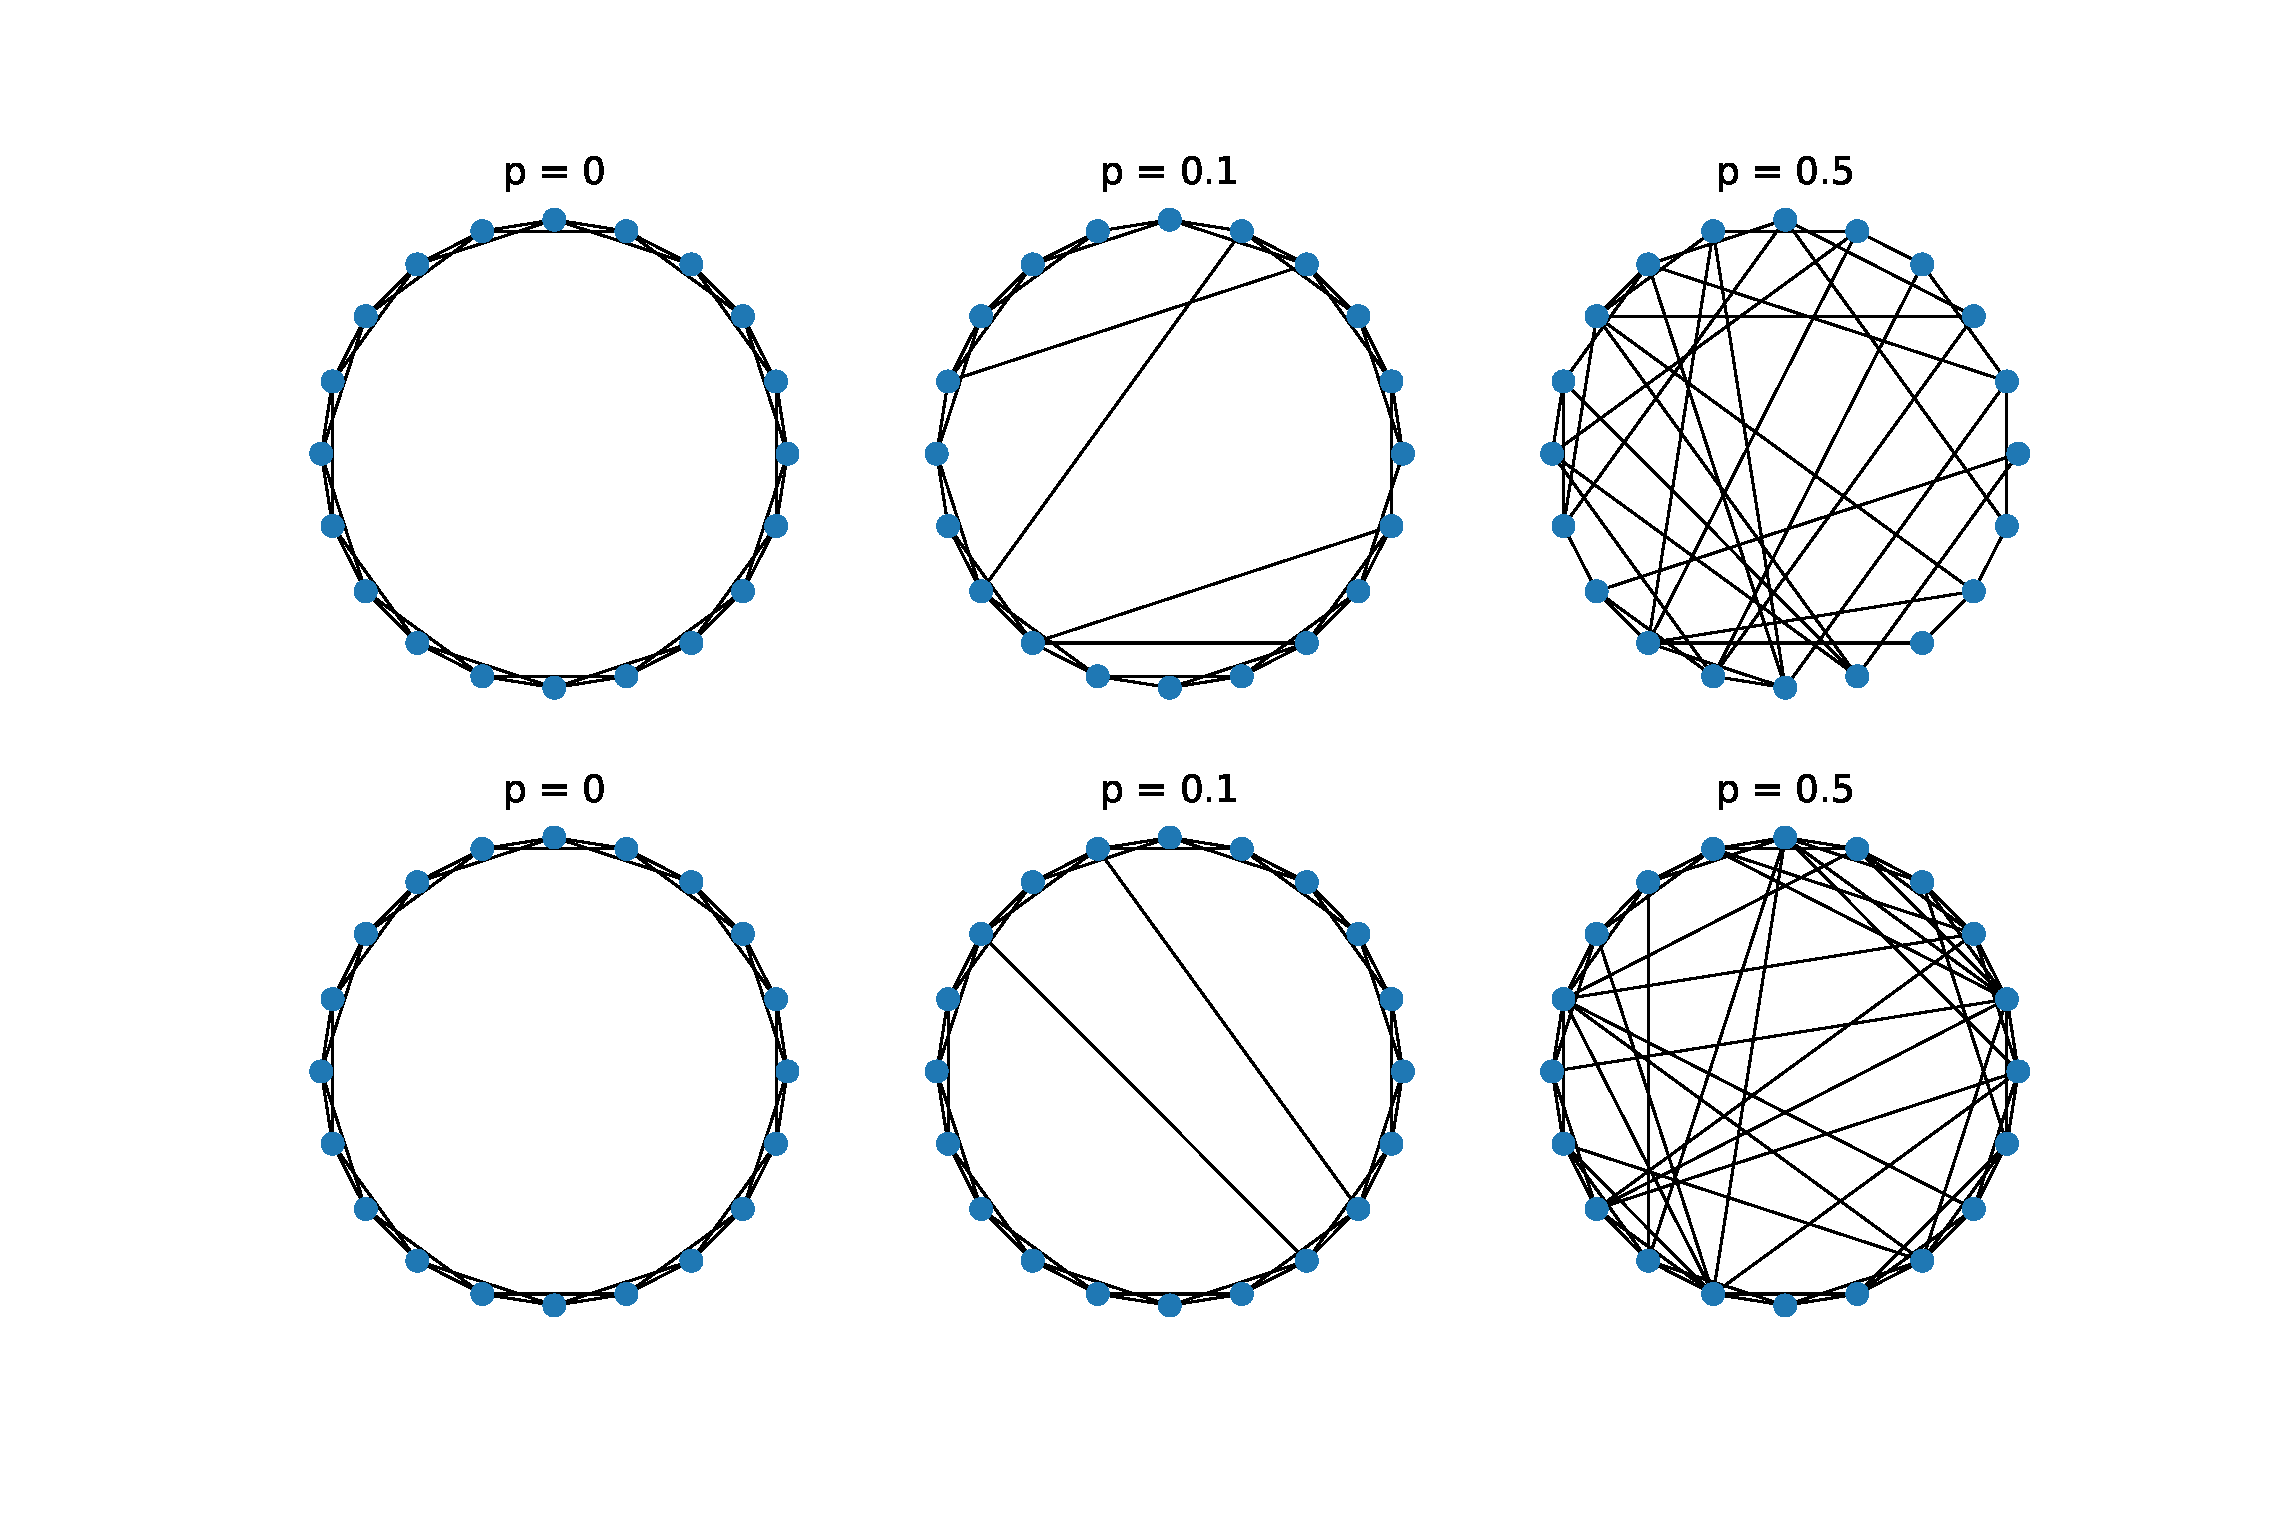
\includegraphics[width = 0.8\textwidth]{small_world_network_model.eps}
    \centering
    \caption{A demonstration of WS model(top) and NW model(bottom). The paramters are: $n=20$, $k=4$, $p=0,0.1,0.5$.}
    \label{fig:small_world_models}
\end{figure}
About 50 years ago, a famous study was carried out by Standley Milgram\cite{milgram1967small} in the interest of this question: how many intermediates are needed to pass a message between two irrelevant or distanced person? This is known as the small-world problem. As counterintuitive as it may seem, the medium number of intermediates needed is only 5(an average of 6)\cite{milgram1967small}. This is not a fair and undoubtable experiment but it is almost impossible to determine the actual number of messengers needed in real world. Nevertheless, this number would be smaller than most peoples' expectation. Mathematically, the small world problem is the study of graphs with small average distance, since network scientists believe that in real world networks, the average distance is small with high average clustering coefficient. Previously, we introduced the formula to calculate the average distance $L_r$ of a random graph. Thus, if a graph has $L/L_r <1$ and $C/C_r>1$, this graph can be considered to have the small-world property.\\
\par
A small-world network can be generated using a Watts-Strogatz(WS) model\cite{wsmodel} or a Newman-Watts(NW) model(a variant of the WS model)\cite{nwmodel}. Both models require three parameters: number of nodes $n$, number of connected closest neighbours $k$ and rewiring probability $p$. The key of both model is rewiring. The graph starts with $n$ nodes, each node is connected to $k$($k-1$ if $k$ is odd) nearest neighbours; $nk/2$ edges will be created. For each edge, there is a proabbility $p$ that this edge will be rewired to another ending node(single link rewiring). While rewiring, the WS model removes the edge $(u,v)$ and add a new edge $(u,w)$. Thus, the number of edges stays the same. However, the NW model maintains the edge $(u,v)$ and adding the new edge $(u,w)$, causing the expectation of number of edges after rewiring to be $nk/2+pnk/2$. Rewiring will add short paths to the networks, and cause the average distance to be exceptionally smaller. Suggested by Barabási\cite{barabási2016network}, to obtain both high clustering and low average distance(properties of a small-world network), $p$ should be between 0.001 and 0.1.\\


\subsection{Scale-free network}
A controversial topic of network science is whether
real networks are usually scale-free\cite{holme2019rare}. To understand what is a scale-free network, we need to scope into the degree distribution of graphs.\\

\begin{figure}[ht]
    \centering
    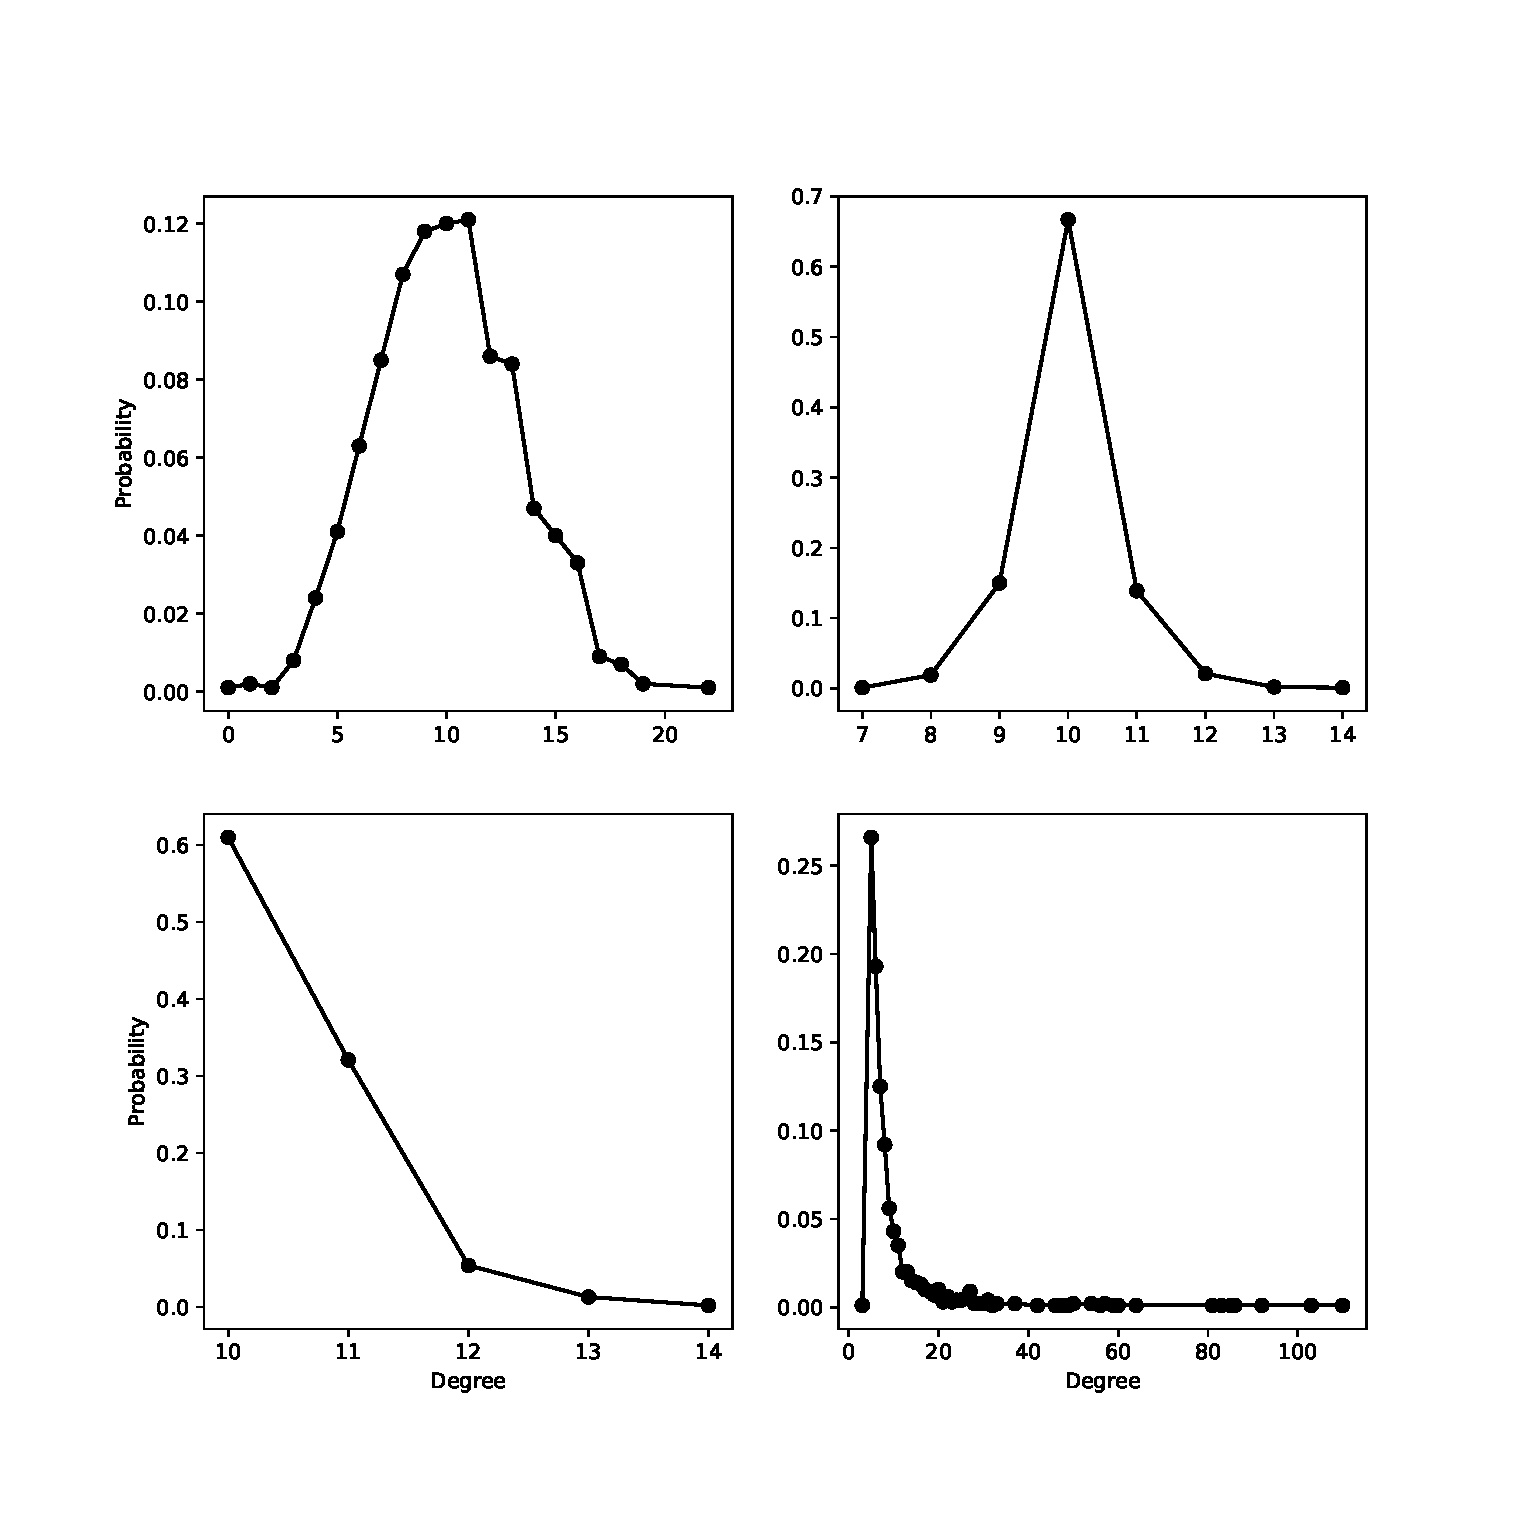
\includegraphics[width=\textwidth]{degree_distribution.eps}
    \centering
    \caption{Degree distribution of a $G(n,m)$ graph with $n=1000,m=5000$ and a graph generated using Barabási-Albert model with $n=1000,m=5$.}
    \label{fig:degree_dist}
\end{figure}

Suggested by Barabási\cite{barabási2016network}, the degree distribution of a random network is expected to follow a binomial distribution. However,it might not be the actual distribution of real networks. A controversial idea that hasn't yet been proven in network science community is: are real networks' degree distribution follows a power-law distribution? A power-law distribution follows: $P(k) \sim k^{-\gamma }$, the parameter $\gamma$ is typically in the range $2<\gamma<3$. If the degree distrution of a network follows a power-law distribution, the network is said to be a scale-free network. Even though there are counter-examples\cite{broido_clauset_2019}, many network scientists still believe that real networks are scale-free\cite{albert1999diameter}. In order to further simulate the behaviour of real networks, Barabási introduced the Barabási-Albert(BA) model to create scale-free networks.\cite{barabási2016network}.\par
The BA model requires two parameters: $n$ and $m$. Initally, only one node is created and $n-1$ nodes will be added to the network consequently. Whenever a node is added into the network, it will connect to $m$ nodes. The logic of connection is the key of this model. Nodes are more likely to connect to nodes with more edges than nodes with less edges. For instance, a node has been added to the network, it is more likely to connect to a node with degree $k=7$ than a node with degree $k=3$. This logic of connection is called preferential attachment. Essentially, like in real world, nodes are more likely to connect to nodes that have more impact on the network.\cite{pa_test} The BA model ensures most of the nodes have low degree, whereas only a few nodes have exceptionally high degree, as shown in figure \ref{fig:degree_dist}. An ideal way to fit the power-law distribution is using a linear regression to fit the data in log-log scale.

\subsection{Generating graphs}
\label{generate_graphs}
All graph models are utilized as below(unless specified):
\begin{itemize}
    \item $G(n,m)$ random graphs/networks or random graphs/networks. With given $n$, $m$ will be randomly selected between $n-1$ to $n(n-1)/2$ to create various networks with different number of $m$.
    \item For WS and NW graphs, three parameters are required. Given parameter $n$, $k$ will be randomly selected between 1 and $(n-1)$ to give a larger range of $m$. $p$ is also randomize, within the range 0.01 and 0.1 to simulate small-world network as mentioned in section \ref{small_world}. By randomize two parameters, more diversity samples will be generated.
    \item Two parameters are needed for BA graphs, given $n$, $m$ will be randomize between 1 and $(n-1)$, so we can generate samples with different number of edges.
\end{itemize}

\section{Methods}
\subsection{Implemeted methods}
In this project, 8 methods will be introduced, 7 of them are based on paper pubilished\cite{KIM20082637}\cite{odc}, and a new measure $MA_{RI}$ will be introduced. $MA_{RI}$ is based on the idea of $MA_g$, and it also performs similarly.\par
To compare complexities, all complexities should be normalised within range $0<complexity<1$. Hence, finding the upper bound and lower bound of each complexity is essential, even though the lower bound for most measures is 0.
\begin{itemize}
    \item Subgraph measures:
    \begin{itemize}
        \item $C_{1e,st}$
        \item $C_{1e,spec}$
        \item $C_{2e,spec}$
    \end{itemize}
    \item Product measures:
    \begin{itemize}
        \item $MA_g$
        \item $MA_{RI}$
        \item $Cr$
        \item $Ce$
    \end{itemize}
    \item $OdC$ (Entropy measure)
\end{itemize}
\subsection{Different subgraph measures}
Definition of subgraph was introduced in section \ref{graph}, so a intuitive idea of measure is to count the number of different subgraphs in a given graph. The question is: how to count subgraphs and how to determine whether they are truly identical or not? Different subgraphs can be created using edge deletion. There are two approaches in this project: removing one edge or remove two edges. Removing more edges is not optimal considering the complexity of calculation. Deleting one edge from a graph with $m$ edges will result in $m$ subgraphs, or ${m \choose 2}$ using two edges deletion. After obtaining $m$ or ${m \choose 2}$ subgraphs, the next step is to find number of unique subgraphs. Two identical subgraphs are said to be isomorphic. To determine isomophicness, there are two possible methods.\par
The first approach is to find out the number of spanning tree of a subgraph. A spanning tree contains all the nodes in a subgraph with minimum number of edges. This can be calculated using the Kirchkoff's theorem\cite{priezzhev1985dimer}: number of spanning tree = cofactor of Laplacian matrix $L$. By counting different number of spanning trees, isomorphicness can be determined: two subgraphs wtih same $m$ ,$n$ and same number of spanning trees are isomorphic. This is a computationally cheaper approach with possible errors. A more complex but precise way to determine isomorphicness is to compare the spectrum of Laplacian matrix of subgraphs. Calculating and comparing both Laplacian matrix and signless Laplacian matrix(all entries are positive or 0) will offer a better result. If two subgraphs with same spectrum on both Laplacian matrix and signless Laplacian matrix, they are isomorphic. As mentioned, the complexity need to be normalised to allow comparison. A good upper bound for both edge deletion method is $m_{cu}=n^{1.68}-10$.\cite{KIM20082637}.Three measures can be defined:
\begin{itemize}
    \item $N_{1e,st}$, the number of different subgraphs with different number of spanning trees, after cutting one edge. The normalised complexity $C_{1e,st} = (N_{1e,st}-1)/(m_{cu}-1)$.
    \item $N_{1e,spec}$, the number of different subgraphs with different spectrums, after cutting one edge. The normalised complexity $C_{1e,spec} = (N_{1e,spec}-1)/(m_{cu}-1)$.
    \item $N_{2e,spec}$, the number of different subgraphs with different spectrums, after cutting two edges. The normailised complexity $C_{2e,spec} = (N_{2e,spec}-1)/({m_{cu} \choose 2}-1)$.
\end{itemize}

\subsection{Potential problems and solutions of different subgraph measures}
\label{problem}
During the implementation of different subgraph measures, problems were found, possible solutions are also given for future implementation.\\
Different subgraph measures are principally simple, but they are complex to compute, within at least $O(n^2)$ time\cite{KIM20082637}. This is not the only problem. An upper bound of the complexity $m_{cu} = n^{1.68}-10$ was assumed by Kim and Wilhelm\cite{KIM20082637} to normalise the complexity. However, from the simulation, we found that this may not be the actual upper-bound of the different subgraph measures.

\begin{figure}[ht]
    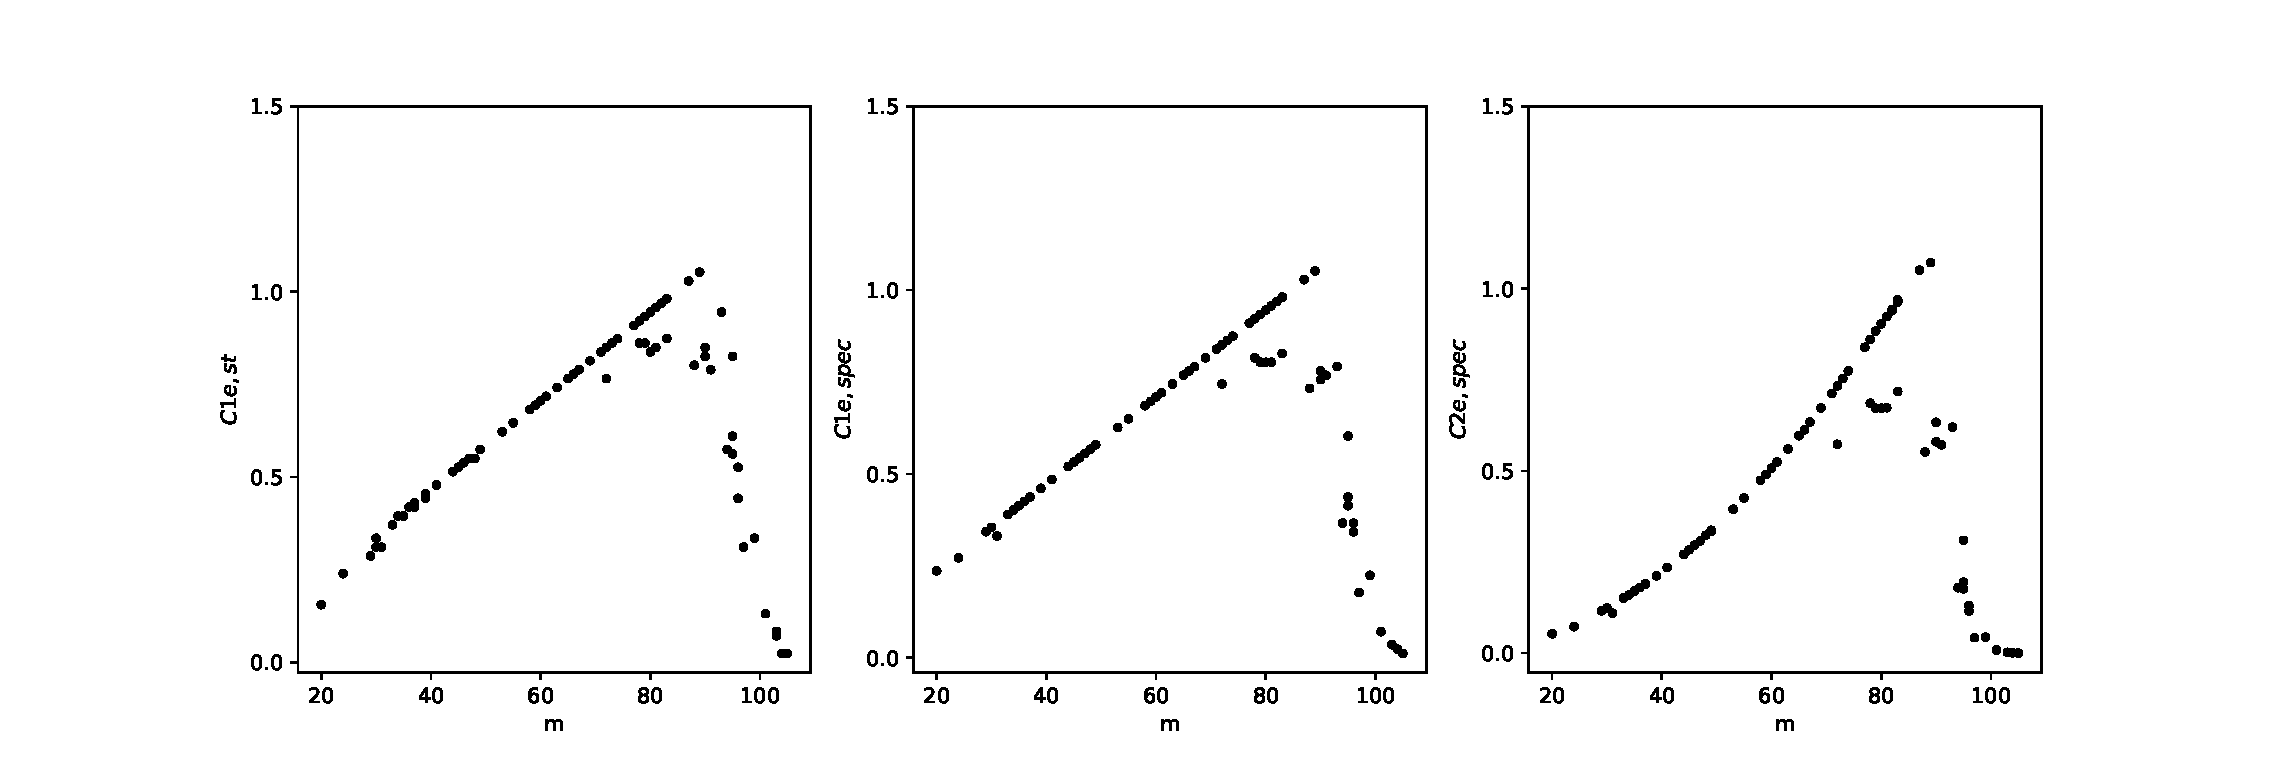
\includegraphics[width=\textwidth]{subgraph_measures.eps}
    \caption{Different subgraph measure of 1000 $G(n,m)$ random graphs, with $n$ = 15.}
    \label{fig:subgraph_measure}
\end{figure}

The complexity is abnormal for graphs with around 90 edges and 15 nodes as shown in figure \ref{fig:subgraph_measure}. This could imply that the upper bound assumption $m_{cu}$ is not correct, but there is another possible reason, which is the problem of floating point arithmetic.\par
On most machines today, numbers are represented in binary system\cite{floating_point}. For example, 0.2 is recorded as 0.00110011001100110011... in a binary system. This series is infinite, represented by $1*2^{-3}+1*2^{-4}+1*2^{-7}+1*2{-8}...$. For obvious reasons, computer scientists don't want to work with infinite series, therefore, the series is approximated. On a modern compueter, the series is usually approximated to 63 digits with 1 digit represents the sign of the number. After approximation, the error could cause the equal operation to fail. A well known example is that for modern programming language or machine that operates this numbering system, 0.2+0.1 does not equal to 0.15+0.15. As a result, the inaccurate comparison may cause more number of different subgraphs than actual.\par
The core of different subgraph measure is to compare the cofactor($C_{1e,st}$) or spectrum($C_{1e,spec}$ and $C_{2e,spec}$) of a subgraph. Given the fact that the proabbility of a decimal number to appear in the sprectrums is high and the cofactor might exceed the upper bound of numbering system\cite{python_int}. The comparisons will be inaccurate with a high probability. There are three possible solutions:
\begin{itemize}
    \item As suggested, errors will be made when approxiamted by the machine. An error threshold can be used when comparing spectrums and cofactors. For example, two numbers with relative error less than 1\% can also be considered as equal numbers. One disadvantage is the increase of complexity, taking more time and effort to compare the spectrums/number of spanning trees.
    \item Similarly, numbers can be rounded before comparison to avoid error. This is used in the implementation of different subgraph measures, all cofactors and spectrums are rounded to first 10 significant figures. This solution requires less computation time than first solution and reduce the number of misclassification. The drawback is that similar graphs can be considered as isomorphic graphs, this also applies to the first provided solution, but with higher accuracy for large graphs. This may still gives complexities larger than 1, but it is the best solution considering the effort spent. Thus, this solution iwll be used in this project.
    \item Instead of using $m_{cu}$ as the upper bound, $m$ or $n(n-1)/2$ can be used for one-edge-deleted subgraph complexity and $\genfrac(){0pt}{2}{m}{2}$ for two-edges-deleted subgraph complexity. This gurantees the normalisation and avoid the mistake that caused by the first two solutions, but on the other hand, causing the complexity to be different.
\end{itemize}
\par
A unique problem with $C_{2e,spec}$ is the value is not properly scaled for small graphs.

\begin{figure}[ht]
    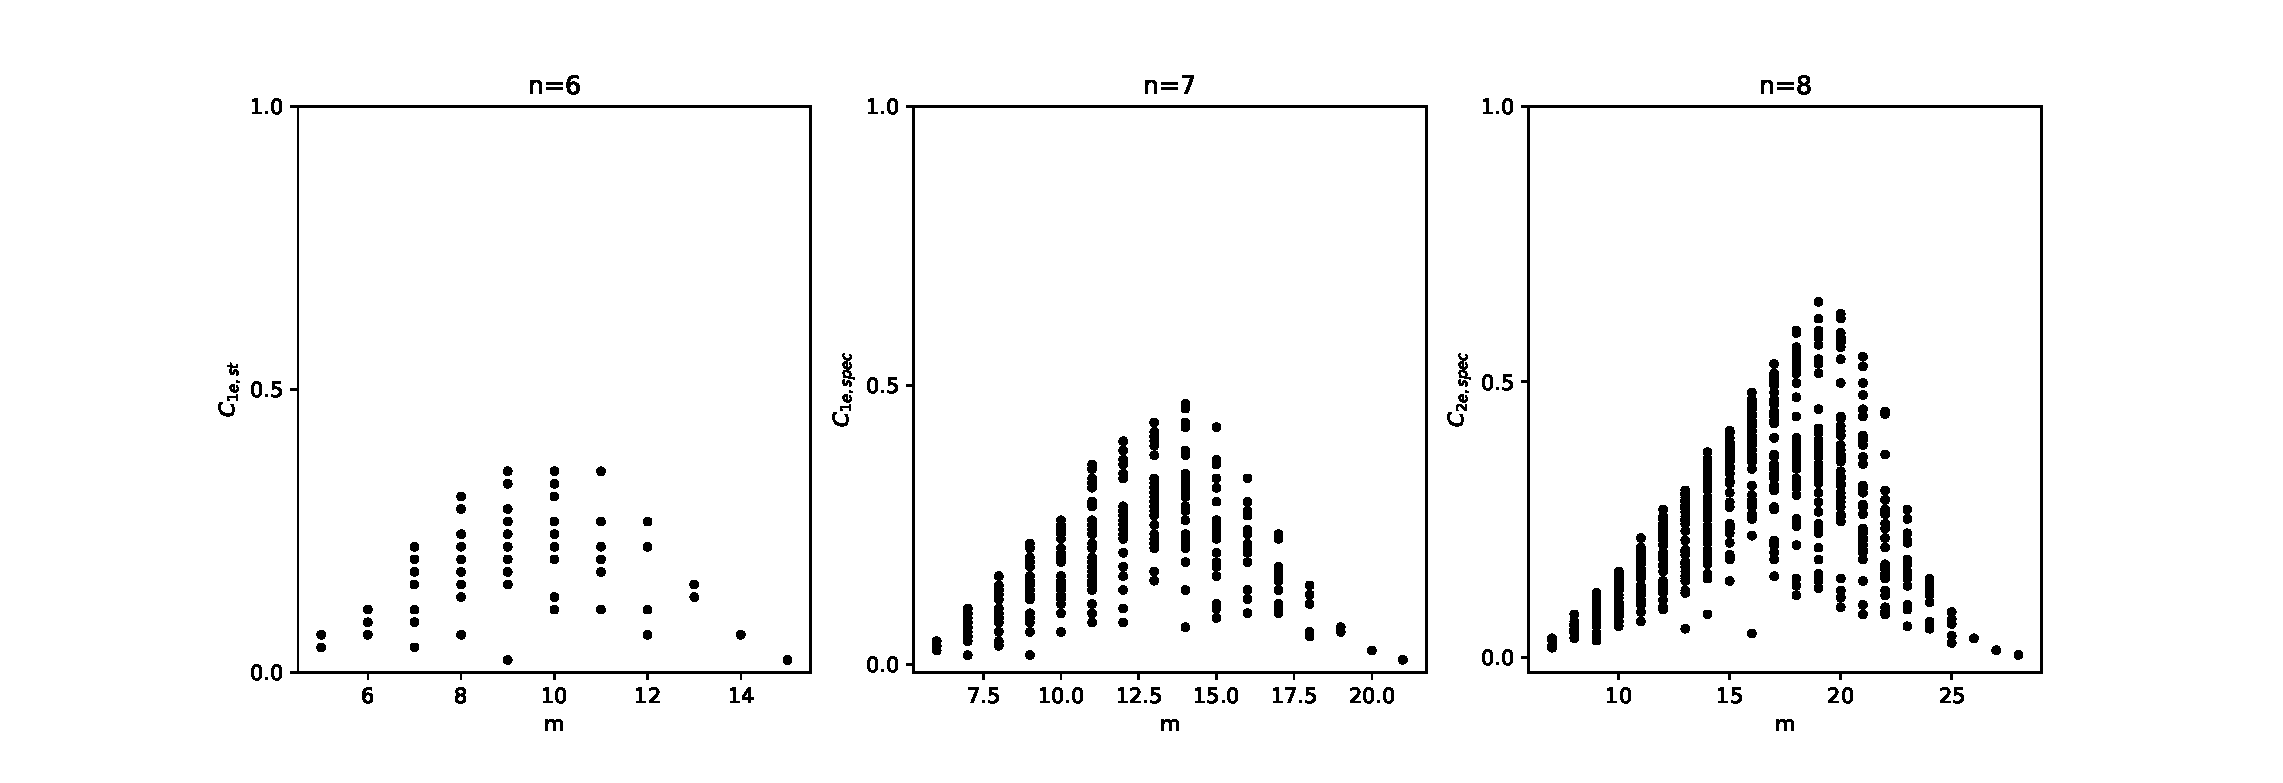
\includegraphics[width = \textwidth]{c2espec.eps}
    \caption{$C_{2e,spec}$ complexities of $G(n,m)$ random graphs for n = 6,7,8 respectively. For each $m$, 50 samples are generated}
    \label{fig:c2espec}
    \centering
\end{figure}
\par
The upper-bound of $C_{2e,spec}$ is 0.5 while $ n\leq7 $. To have an upper-bound at 1, the complexity values have to be scaled by 2. However, scale by 2 will cause the complexity to exceed 1 for larger graphs. Thus, we sticked to the original normalisation and scaling, $C_{2e,spec}$ will have an upperbound at 0.5 for $n=7$, and less for smaller $n$s.

\subsection{Product measure}
The core idea of product measure is to assign low complexity at both extremes(path and cliques) and higher complexity to graphs with medium number of edges.
\subsubsection{Medium articulation for graphs($MA_g$)}
\label{magdefinition}
This measure is based on redundancy and mutual information of a graph.\cite{wilhelm2007information} The unnormalized complexity can be defined as the product of redundancy and mutual information $C=R*I$, with redundacy $R=\frac{1}{m}\sum_{i,j>i}ln(d_id_j)$ and mutual information $I=\frac{1}{m}\sum_{i,j>i}ln(\frac{2m}{d_id_j})$. The core of this measure is the variable $d_id_j$. It is product of degree of two nodes. This variable will be maximised when the graph is fully connected(clique) and minimized when the graph is least sparse and highly ordered(path).
\begin{itemize}
    \item Highest redundancy: $R_{clique} = 2ln(n-1)$
    \item Lowest redundancy: $R_{path} = 2(\frac{n-2}{n-1})ln(2)$
    \item Highest mutual information: $I_{path} = ln(n-1)-(\frac{n-3}{n-1})ln2$
    \item Lowest mutual information: $I_{clique}=ln(\frac{n}{n-1})$
\end{itemize}
\par
Since the maximum and the minimum of redundancy and mutual information can be found, normalization technique can be applied to ensure the complexity $MA_g$ is bounded by 0 and 1.
\begin{equation}
    MA_g=MA_R*MA_I,
\end{equation}
with:
\begin{equation}
    MA_R=4(\frac{R-R_{path}}{R_{clique}-R_{path}})(1-\frac{R-R_{path}}{R_{clique}-R_{path}})
\end{equation}
\begin{equation}
    MA_I=4(\frac{I-I_{clique}}{I_{path}-I_{clique}})(1-\frac{I-I_{clique}}{I_{path}-I_{clique}})
\end{equation}
\subsubsection{Efficentcy complexity($Ce$)}
Efficiency complexity is based on the efficiency of adding shorter path in a network.\cite{latora2003economic} As suggested in section \ref{small_world}, adding short paths will significantly shorter the average shortest distance in a network. However, adding more paths will cost energy. The ratio between shorten distances and cost of energy is defined as the efficiency. A complex graph should maintain short average distance and low energy used as possible. The efficiency is calculated as $E=\frac{1}{n(n-1)/2}\sum_{i,j}\frac{1}{d_i,j}$. To normalise the complexity, identify the lowest graph with lowest efficiency, a path, is: $E_{path} = 2/(n(n-1))\sum_{i=1}^{n-1}(n-i)/i$. Consequently, the normalised complexity is $C_e=4(\frac{E-E_{path}}{1-E_{path}})(1-\frac{E-E_{path}}{1-E_{path}})$

\subsubsection{Graph index complexity($Cr$)}
In section \ref{graph}, Laplacian matrix was introduced. $Cr$ is depending on another graph matrix which is called adjacency matrix. The adjacency matrix is essentailly Laplacian matrix with all diagonal elements being 0. This records all the edges within the network. Using previous studies, all eigenvalues of the adjacency matrix are real.\cite{brouwer2011spectra} The largest eigenvalue is also knows as the index $r$. To normalise the complexity, $r$ is found out that $2cos(\pi /(n+1) \leq r \leq n-1)$.\cite{brouwer2011spectra} Therfore, a normalised complexity can be constructed, which is given by: $Cr=4c_r(1-c_r)$ with $c_r=\frac{r-2cos(\pi /(n+1))}{n-1-2cos(\pi /(n+1))}$.

\subsection{Offdiagonal complexity($OdC$)}
A node-node link correlation matrix need to be constructed to calculate $OdC$.\cite{odc} The matrix element $c_{i,j}$ records the number of neighbours with degree $j \geq i$ of all nodes with degree $i$. $OdC$ assigns higher complexity to graphs that their nodes have no preferences on their neighbours degree. A vector $a_n$ is calcualted by summing up all the rows in the matrix. The normalised $OdC$ is calculated as:\\
$OdC=-(\sum^{k_{max}-1}_{n=0}A_nln(A_n))/ln(n-1)$ with $A=a_n/\sum_{n=0}^{k_{max}-1}a_n$(proability of each $a_n$).
\subsection{$MA_{RI}$}
$MAg$ measure is a product measure, which assigns higher complexity to graphs with medium number of edges and lower complexity at both extremes(path and clique). Using the product of redundancy $R$ and mutual information $I$, with normalisation, $MAg$ is defined as\cite{KIM20082637}:
\begin{equation}
    \label{eq:RandI}
    \begin{gathered}
        R = \frac{1}{m}\sum_{i,j>i}ln(d_id_j)\\
        I = \frac{1}{m}\sum_{i,j>i}ln(\frac{2m}{d_id_j})\\
    \end{gathered}
\end{equation}
\begin{equation}
    \label{eq:mag}
    \begin{gathered}
        MA_R = 4(\frac{R-R_{path}}{R_{clique}-R_{path}})(1-\frac{R-R_{path}}{R_{clique}-R_{path}})\\
        MA_I = 4(\frac{I-I_{clique}}{I_{path}-I_{clique}})(1-\frac{I-I_{clique}}{I_{path}-I_{clique}})\\
        MA_g = MA_R * MA_I
    \end{gathered}
\end{equation}
$I$ can be written as:
\begin{equation}
    \begin{gathered}
        \label{eq:rewriteI}
        I = \frac{1}{m}\sum_{i,j>i}ln(\frac{2m}{d_id_j})\\
        I = \frac{1}{m}(\sum_{i,j>i}ln(2m)-\sum_{i,j>i}ln(d_id_j))\\
        I = \frac{1}{m}\sum_{i,j>i}ln(2m)-\frac{1}{m}\sum_{i,j>i}ln(d_id_j)\\
    \end{gathered}
\end{equation}
\begin{equation}
    \label{eq:mutual_info}
    I = ln(2m)-R
\end{equation}
\par
$R_{path},R_{clique},I_{path}$ and $I_{clique}$ represent the lowest redundacy, highest redundancy, highest mutual information and lowest mutual information of graphs with fixed $n$ respectively. The equations can be found in section \ref{magdefinition}. Kim and Wilhelm suggested that network scientists may use $C=(R-R_{path})(I-I_{clique})$ as a complexity meassure, however, the upper bound cannot be found to normliase the complexity \cite{KIM20082637}. From our study, an upper bound of $C$ can be calculated analytically.\par
Assuming the upper bound $C_{max}$ can be found, $0<C/C_{max}<1$. As suggested in equation \ref{eq:mutual_info}, $I = ln(2m)-R$, we can rewrite the complexity equation:\\
\begin{equation}
    \label{eq:rewrite_complexity}
     C = (R-R_{path})(ln(2m)-R-I_{clique})\\
\end{equation}
\begin{equation}
    \label{eq:rewrite_complexity_1}
    C = -R^2+(ln(2m)-I_{clique}+R_{path})R+(-R_{path}ln(2m)+R_{path}I_{clique})
\end{equation}
\par
Refereing to equation \ref{eq:rewrite_complexity_1}, the complexity function is a quadratic function with only variable $R$, which means, there is one and only one extreme. Considering the nature of product measure, it is safe to assume that the extreme is a maxima. To find the maxima, differentiates the function respect to $R(R_{max})$ where the function's slope is 0:
\begin{equation}
    \label{eq:mari_diff}
        \frac{dC}{dR} = -2R_{max}+ln(2m)-I_{clique}+R_{path} = 0\\
\end{equation}
\begin{equation}
    \label{eq:rmax}
    R_{max} = \frac{ln(2m)-I_{clique}+R_{path}}{2}
\end{equation}
\par
Even without assumption, $d^2C/dR^2 = -2$ implies the extreme is a maxima. As $C_{max}$ is found, substitutes equation \ref{eq:rmax} into equation \ref{eq:rewrite_complexity}:\\
\begin{equation}
    \begin{gathered}
        C_{max} =(R_{max}-R_{path})(ln(2m)-R_{max}-I_{clique})\\
        C_{max} = (\frac{ln(2m)-I_{clique}+R_{path}}{2}-R_{path})(ln(2m)-\frac{ln(2m)-I_{clique}+R_{path}}{2}-I_{clique})\\
        C_{max} = (\frac{ln(2m)-I_{clique}-R_{path}}{2})(\frac{ln(2m)-R_{path}-I_{clique}}{2})\\
    \end{gathered}
\end{equation}
\begin{equation}
    \label{c_max}
    C_{max} = \frac{(ln(2m)-I_{clique}-R_{path})^2}{4}
\end{equation}
\noindent
Thus, using equation \ref{c_max}, a new normalized measure $MA_{RI}$ can be defined using $C/C_{max}$:\\
\begin{equation}
    MA_{RI} = \frac{4(R-R_{path})(I-I_{clique})}{(ln(2m)-I_{clique}-R_{path})^2}
\end{equation}
\begin{figure}[h]
    \centering
    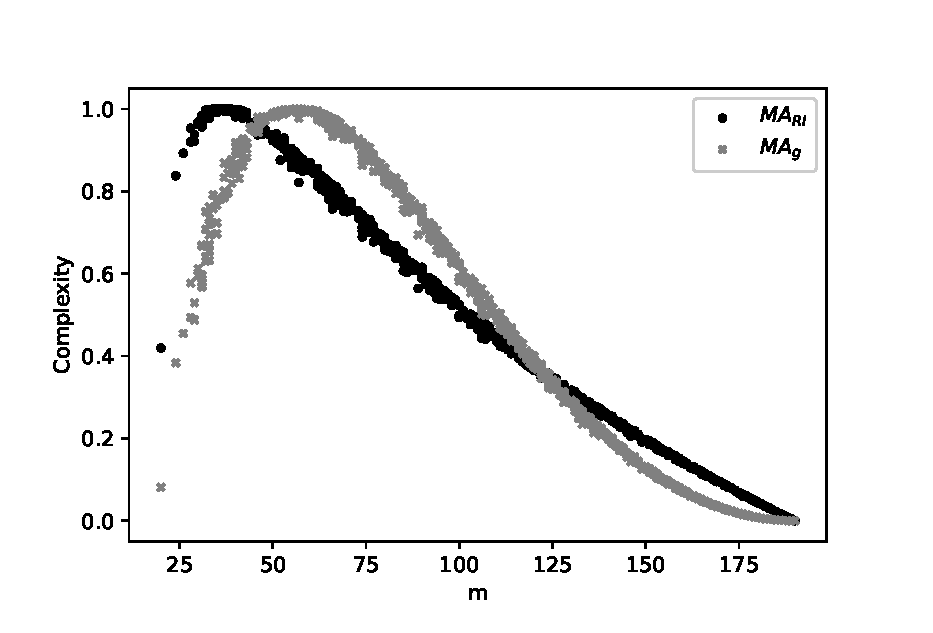
\includegraphics[width=0.7\textwidth]{mariandmag.eps}
    \caption{$MA_g$ and $MA_{RI}$ complexity of $G(n,m)$ networks, all networks have 20 nodes and 1000 samples with random $m$ have been generated.}
    \label{fig:marimagcompare}
\end{figure}
\par
As shown in figure \ref{fig:marimagcompare}, $MA_{RI}$ gives higher coplexity to sparser graphs but less complexity when approaching to medium number of links. Additionally, it decreases more linear and smoothly compare to $MA_g$.

\section{Result}
\subsection{Complexity measures on small random graphs}
\label{complexity}
To validate implemented measures, all measures are applied on $G(n,m)$ random graphs, with $n=7$ and 50 sampels are generated for each $m$. As shown in figure \ref{fig:small_graphs}, we reproduced results as Kim and Wilhelm did in \cite{KIM20082637}. Except $C_{2e,spec}$, as mentioned in section \ref{problem}, there is a scaling problem. Most of the methods reaches its maximum briefly before medium number of edges. Low complexity are given to highly connected graphs and sparse graphs as expected.\par
\clearpage
\newpage
\begin{figure}[p!]
    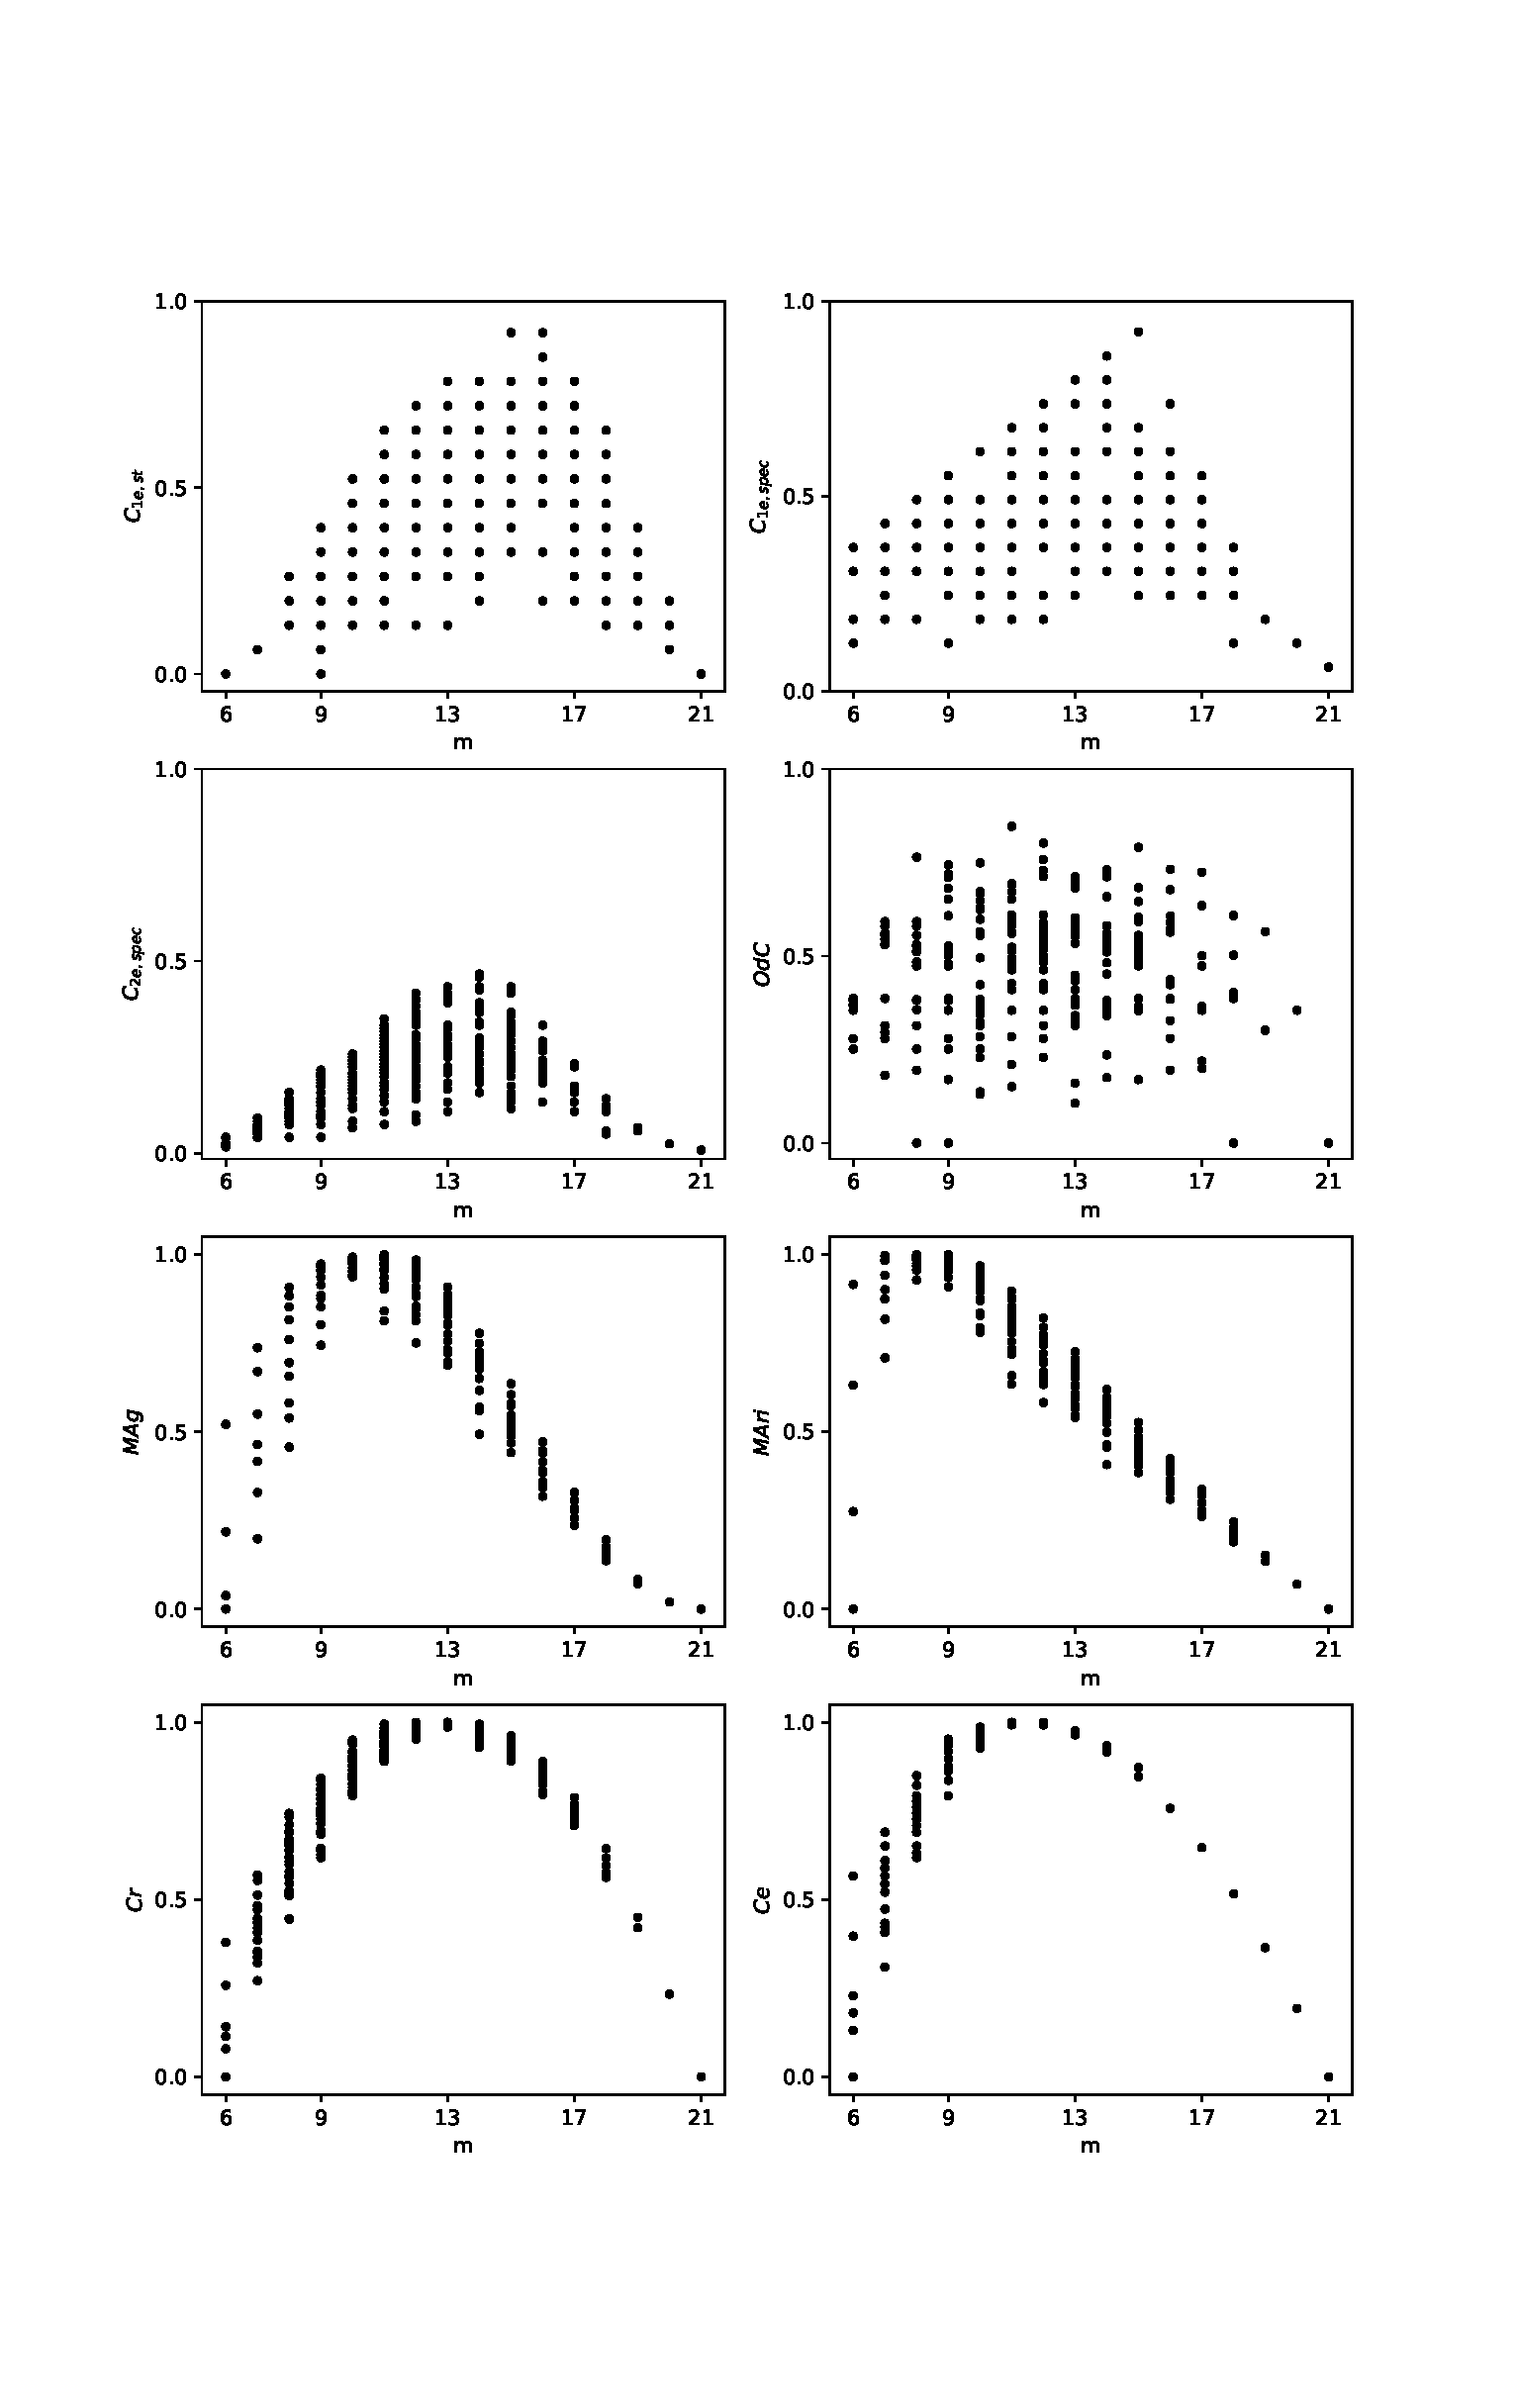
\includegraphics[width=0.85\textwidth]{complexities.eps}
    \vspace*{-0.8in}
    \centering
    \caption{Complexity of graphs generated using $G(7,m)$ model, 50 samples are generated for each $m$. Methods from top-left to bottom-right are: $C_{1e,st}$, $C_{1e,spec}$, $C_{2e,spec}$, $OdC$, $MAg$, $Cr$, $Cr$ and $MAri$.}
    \label{fig:small_graphs}
    \clearpage
\end{figure}
\noindent
\newpage
\begin{figure}[p!]
    \centering
    \vspace*{-2in}
    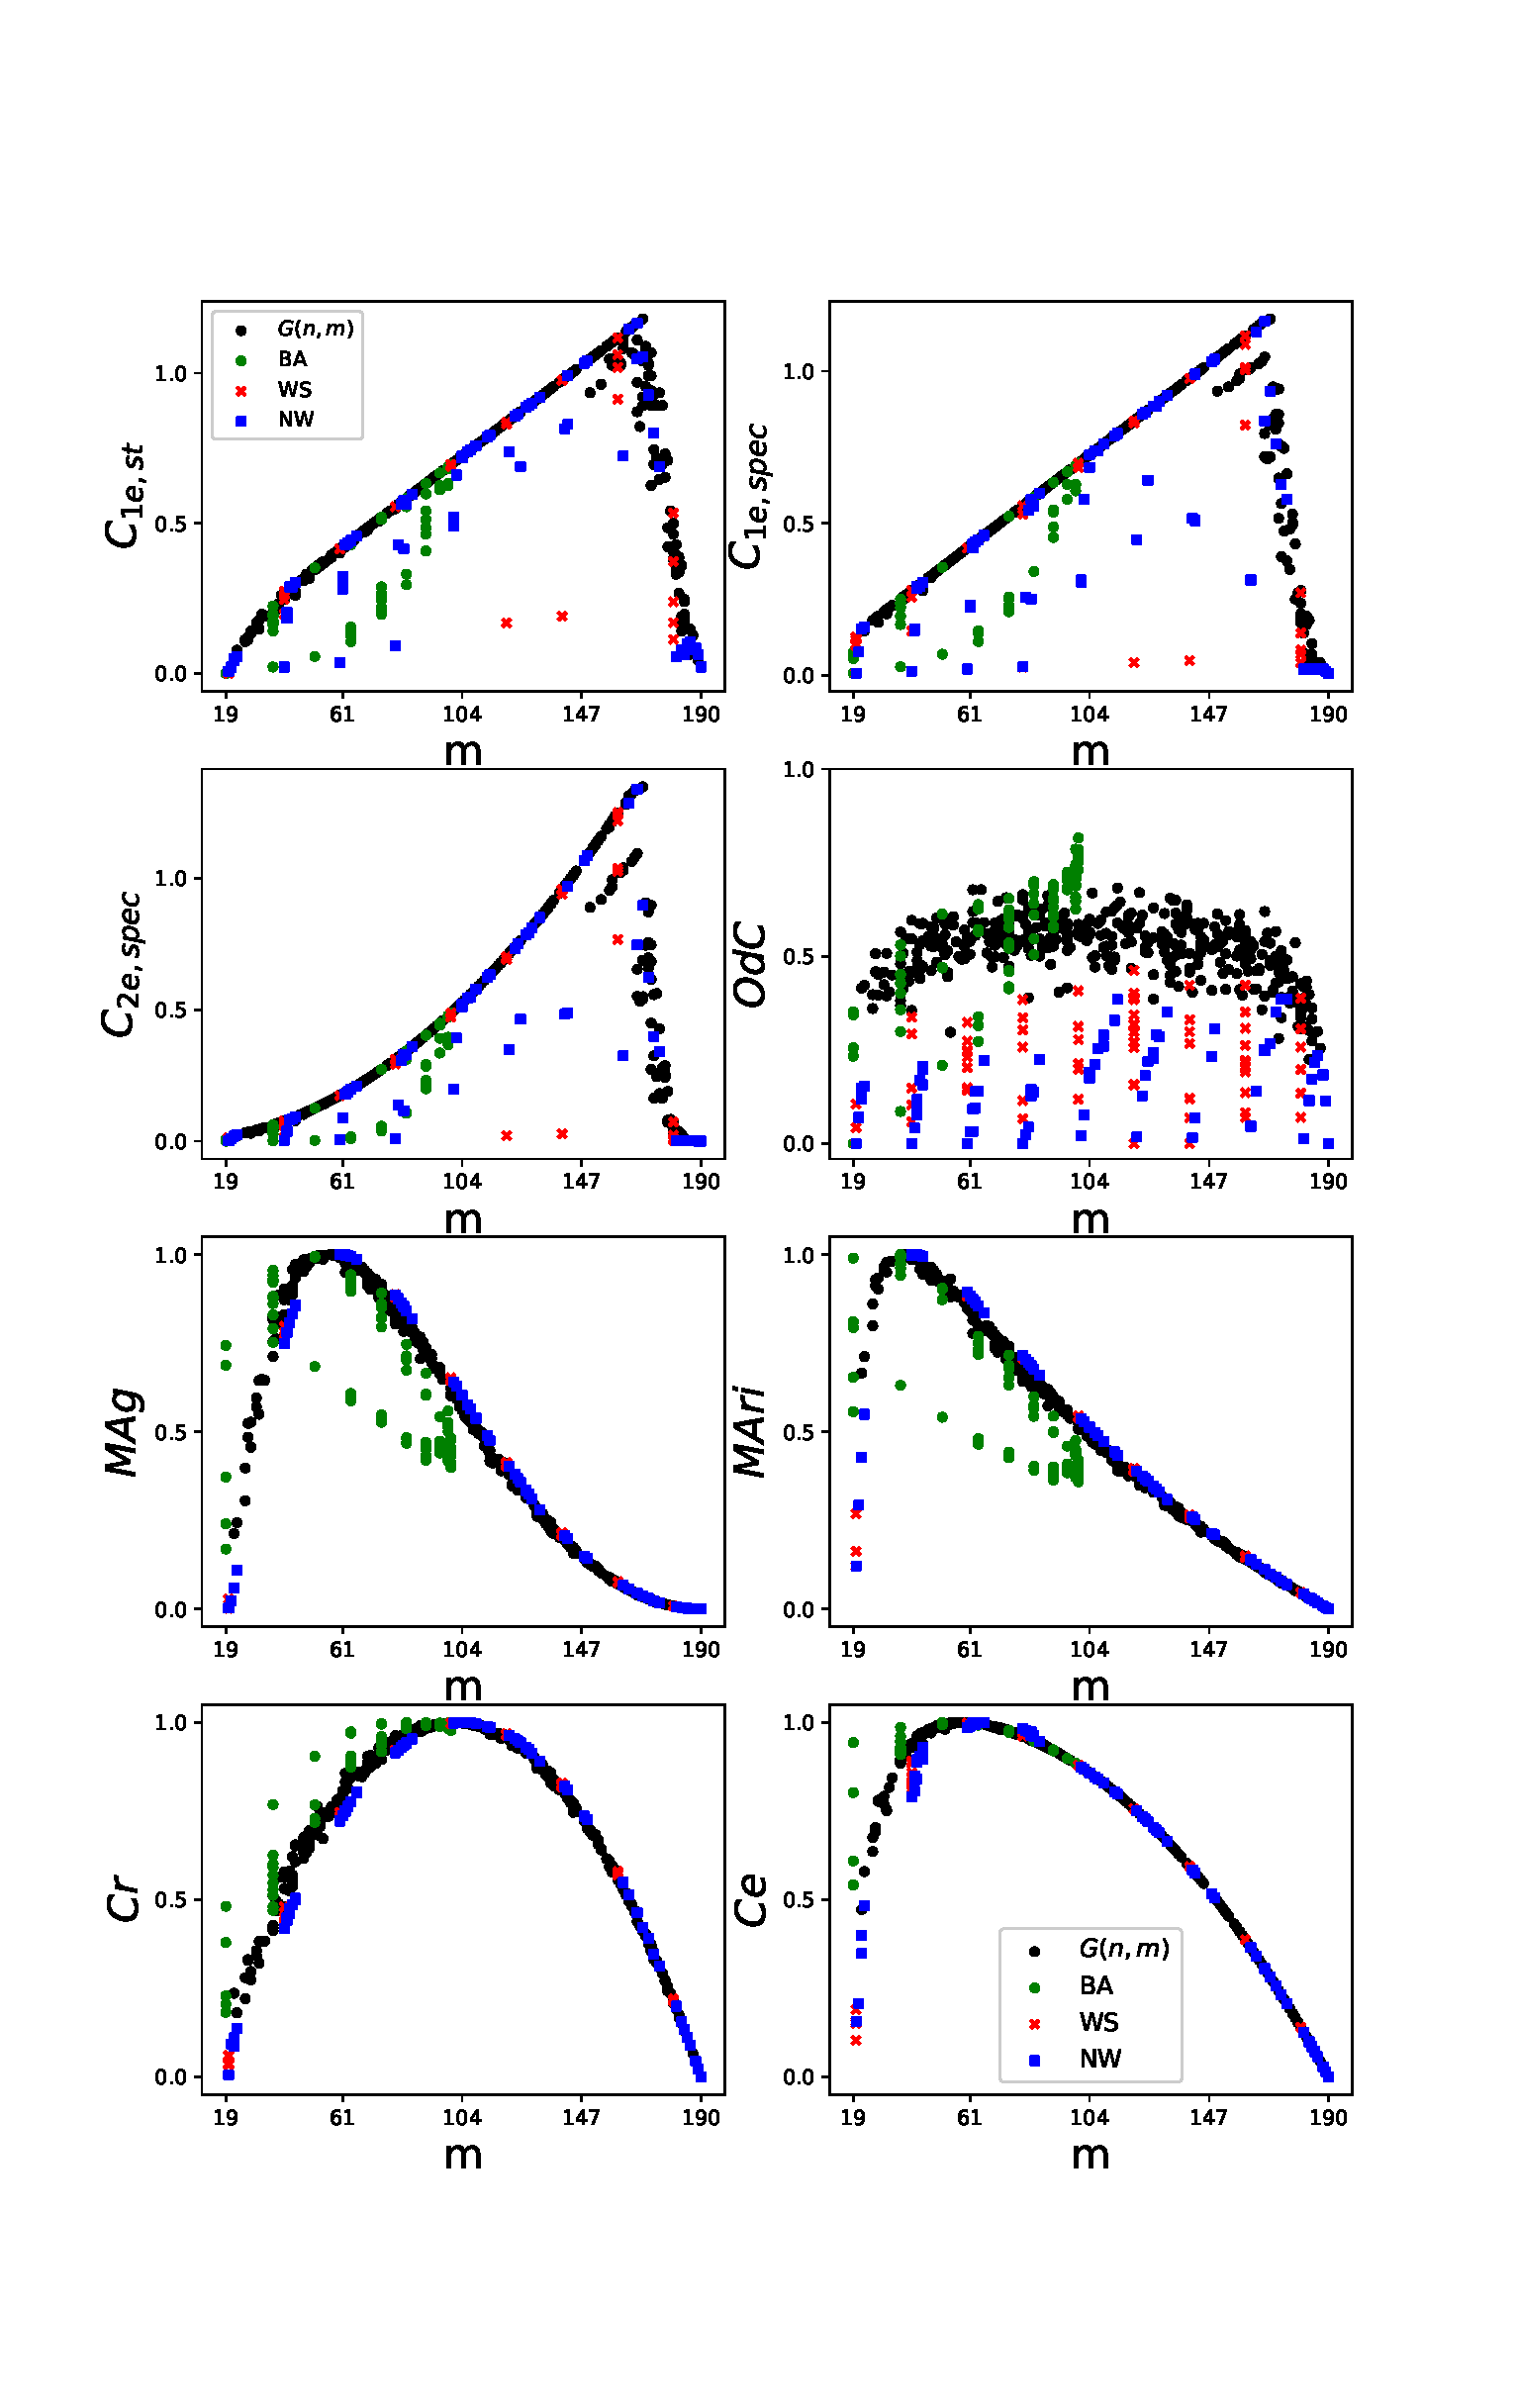
\includegraphics[width = 0.85\textwidth]{complexities_sp.eps}
    \vspace*{-0.8in}
    \caption{Complexity of 500 $G(n,m)$ graphs, 100 BA graphs, 100 WS graphs and 100 NW graphs, with $n=20$. Graphs are generated according to section \ref{generate_graphs}.}
    \label{fig:graph_models}
\end{figure}

Different subgraph measures perform similarly when the graph is neither sparse or strongly connected, there is a big difference between the maximum and minimum with same $m$. Thus, it is very difficult to predict the complexity of a graph with given $m$ and $n$. The highest complexity is reached at $m=15$ for $C_{1e,st}$ and $C_{1e,spec}$ and $m=14$ for $C_{2e,spec}$. There is a miss in the plot: $C_{1e,spec}$ and $C_{2e,spec}$ plot does not contain a data point at (6,0). There is a very small proability for $G(n,m)$ model to generate a star graph(n-1 nodes are connected to 1 node, in total of n-1 edges), which will result in 0 complexity using $C_{1e,spec}$ and $C_{2e,spec}$ measure. Uses different subgraph measures for small graphs is optimal as it is relatively independent of $m$, but not for large graphs due to its complexity.\par


$OdC$ is based on the node-node link correlation matrix of a graph.\cite{odc} Thus, it spreads across the space and has little relationship with $m$. $OdC$ assigns a lot of graphs with 6 edges high complexity than desired. $OdC$ is "hierarchy sensitive", it may not create big difference between graphs when the graphs are considerably small.\par

All 4 product measures are similar, gives higher complexity value at medium number of edges and less at both extremes. There is a very small difference between graphs with same number of edges. $Ce$ and $Cr$ tends to give highest complexity to graphs with exactly $n(n-1)/4$ edges, and $MA_{RI}$ and $MA_{g}$ reach their maximum before medium number of edges as expected. Product measure are highly depending on $m$, such that complexity of a graph can be approximated solely based on $m$ and $n$. Network scientists may use machine learning techniques to approximate complexity of a graph using $m$ and $n$ in a small amount of time. On the other hand, product measure may not be optimal because a complexity measure should not solely based on $m$ and $n$, but the overall structure of a network.


\subsection{BA,WS and NW model}
As informed in section \ref{problem}, different subgraph measures have normalisation problem and the complextity would exceed 1.\par
Surprisingly, diffrent subgraph measures and product measures are struggling to seperate random graphs, WS graphs and NW graphs. Only $OdC$ seperates random graphs and WS,NW model by giving random graphs higher complexity than WS and MW model with fixed $m$. This is because $OdC$ awards graphs with complicated degree correlation.\\
More interesting results are obtained from BA graphs. Different subgraph measures assign lower complexity to BA graphs compare to random graphs. This can be caused by the preferential attachment. Preferential attachment ensures most nodes have low degree and builds hubs(nodes with high degree) in the graph. After cutting an edge/two edges between hubs and nodes with small degree, there is a high chance an isomorphic subgraph can be found, thus lower the complexity of the graph. In another word, subgraphs resulted by cutting the edge between hubs and node with small degree are very similar and occassionally isormophic.\par
$MA_g$ and $MA_{RI}$ perform similarly by assigning BA graphs lower value towards medium number of links. Both measures are depening on the variable $\sum_{i,j>i}d_id_j$. BA graphs ususally have less $\sum_{i,j>i}d_id_j$ because they are highly structure, causing less sum than a random graph. Contrarily, $Ce$ and $Cr$ cannot distinguish BA graphs and random graphs. $Ce$ is based on the efficiency of a graph, a highly complex graph should have small average distance with not too much edges simultaneously. BA graph does not perform different than random graphs in $Ce$ measure.\\

\subsubsection{Configuration model}
\label{configuration_model}
As introduced in section \ref{small_world}, a network is said to be scale-free if its degree distribution follows a power law distribution with $2<\gamma <3$. To observe how the change of $\gamma$ would affect the complexity of a network, we need a model that can generate the graph with given $\gamma$. A configuration model \cite{newmanbook} is able to turn a given degree distribution into a graph, which has the exact degree distribution as the given degree series. 
\begin{figure}[h]
    \centering
    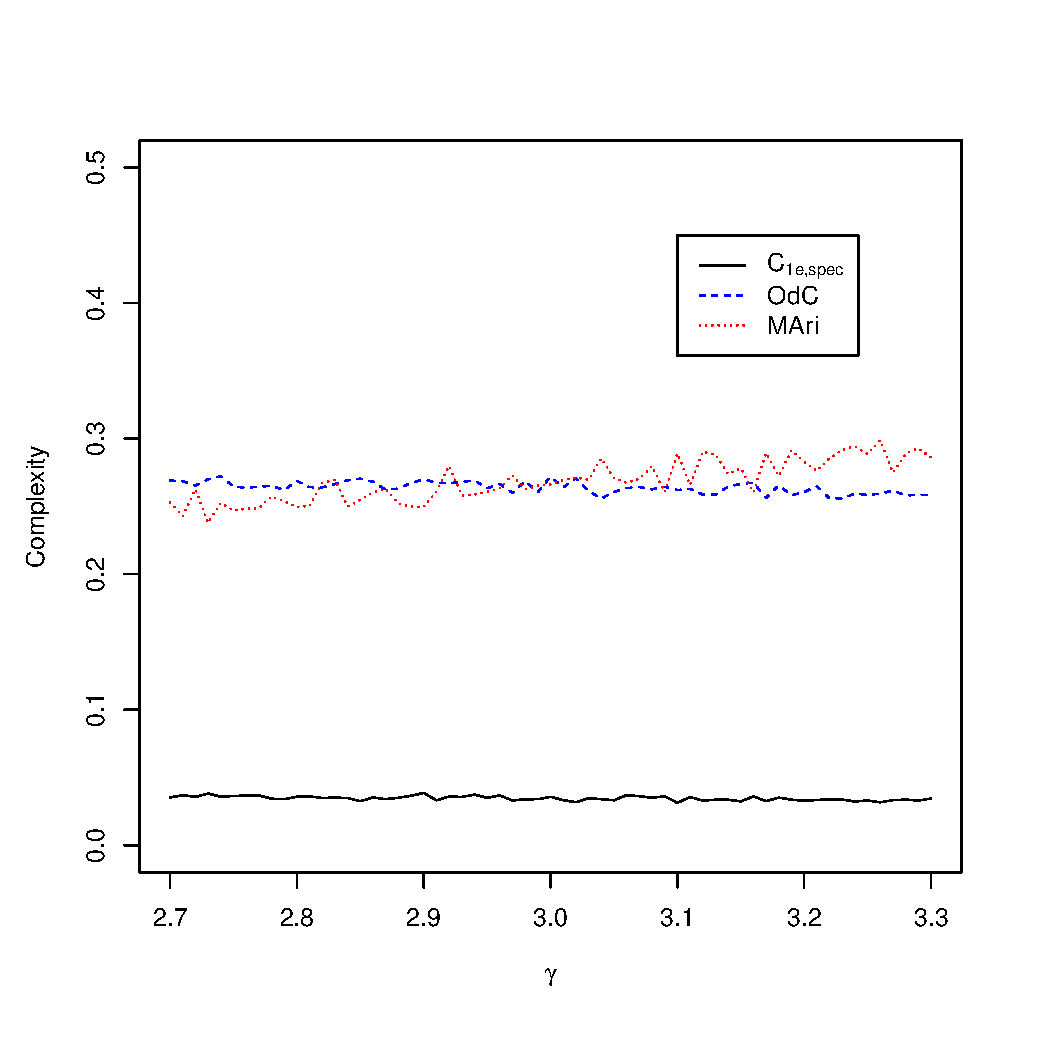
\includegraphics[width=0.6\textwidth]{configuration_model.eps}
    \label{fig:configuration_model}
    \caption{Complexities of graphs generated using configuration model, $n=50$. Results are average of 50 simulations.}
\end{figure}
\par
$OdC$ and $C_{1e,spec}$ didn't change much by varying $\gamma$. $MA_{RI}$ increases slightly as it is very sensitive to the change of degrees of nodes. Overall, varying $\gamma$ does not impact the complexity by a lot. Due to limitation of our implementation, we can only generate a degree distribution within the range $2.7<\gamma<3.3$, by varying $n$ and $\gamma$ in a larger range, and adding a new variable $n$ in the model, it can be more suggestful. 

\subsection{Complexity correlation}
Different type of measures focus on different properties/parameters of a network, monitor the correlation between measures enable further understanding of the properties/parameters each measure is highlighting on. Additioanlly, network scientists may use more than one complexity measure on a network to determine whether they are truly "complex" or not. Combining complexity measures on networks will allow network scientists to comment on the network complexity from different aspect. For these reasons, we choosed three measures($C_{1e,st}$,$OdC$ and $MA_{RI}$) and monitored their behaviours on random and BA graphs. The reason BA graphs are added is to investigate whether distinguish BA graphs and random graphs is possible or not.\\
\begin{figure}[h!]
    \makebox[\textwidth]{
    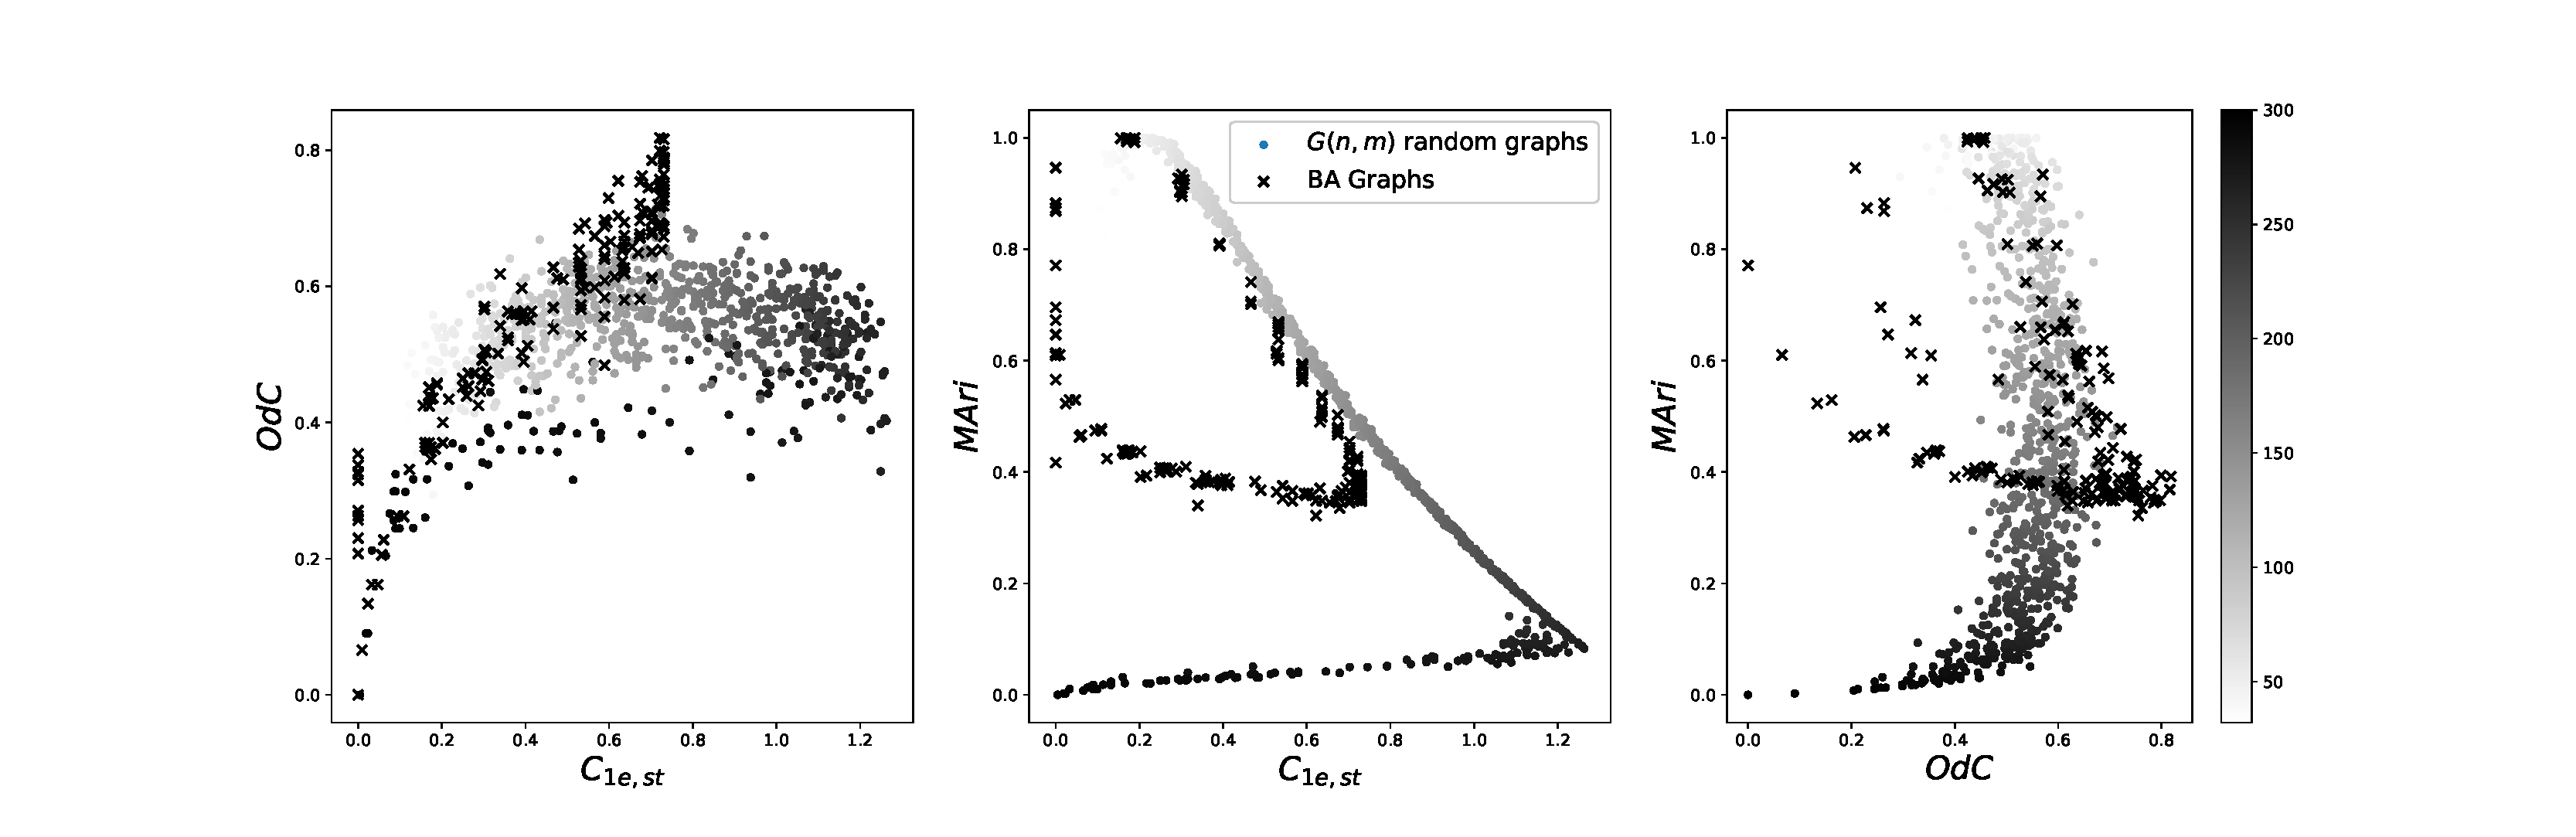
\includegraphics[width = \textwidth]{complexity_correlation.eps}
    }
    \caption{Correation of complexity measures on 1000 random graphs and 200 BA graphs with $n=25$. Generated according to the rules stated in section \ref{generate_graphs}. Colorbar represents change of $m$: higher the $m$, darker the datapoints.}
    \label{fig:correlation}
\end{figure}

\noindent
As figure \ref{fig:correlation} suggests, the correlation between complexity measures are difficult to observe, since they are trying to address different things. As $C_{1e,st}$ value increases, $OdC$ also increases. We indicated in section \ref{complexity}, $m$ is not an important factor for $OdC$. On the other hand, $C_{1e,st}$ is highly based on $m$, the complexity increases linearly with $m$, and then complexity drops quickly after reaching the maximum. By constructing a correlation between $C_{1e,st}$ and $OdC$, seperate BA graphs and random graphs is not possible.\par
Since both complexity measure are heavily depend on $m$, thus we can observe a linear decreasing trend. We can detect a very unique distribution of the BA graphs' complexity: a shape between ellipse and half-moon. This is because both $MA_{RI}$ and $C_{1e,st}$ assign lower complexity values to some of the BA graphs, compare to other BA graphs with same number of edges. Therefore, distinguish Ba graphs and random graphs is difficult.\par
The correlation between $OdC$ and $MA_{RI}$ of random graph seems simple: as $m$ decrease, $MA_{RI}$ decrease speedly but $OdC$ change unnoticeably until the graph is highly connected. On the other hand, the correlation between $OdC$ and $MA_{RI}$ on BA graphs perform slightly different. As suggested, $MA_{RI}$ distributes lower complexity to some BA graphs, and $OdC$ is very consistent. In section \ref{configuration_model}, we did not observe a big change of complexity by varying $\gamma$. To observe a better result, using larger graph is optimal(for instance $n=1000$), but due to technical issues(time complexity), they are not used here.



\subsection{Complement graphs}
Definition of a complement graph is fairly simple: the complement graph contains all the edges that are not in the original graph. To ensure complexity measures can be succesfully applied, graphs that will cause the complement graphs to be disconnected will be removed. Thus, in theory, the original graphs and the complement graphs are not exmtreme graphs. Analysing the complexity correlation between the original graph and the complement graph give us more inspirations of the measure. We have choose three different measures with different types: $OdC$, $MA_{RI}$ and $C_{1e,spec}$.
\begin{figure}[h!]
    \makebox[\textwidth]{
    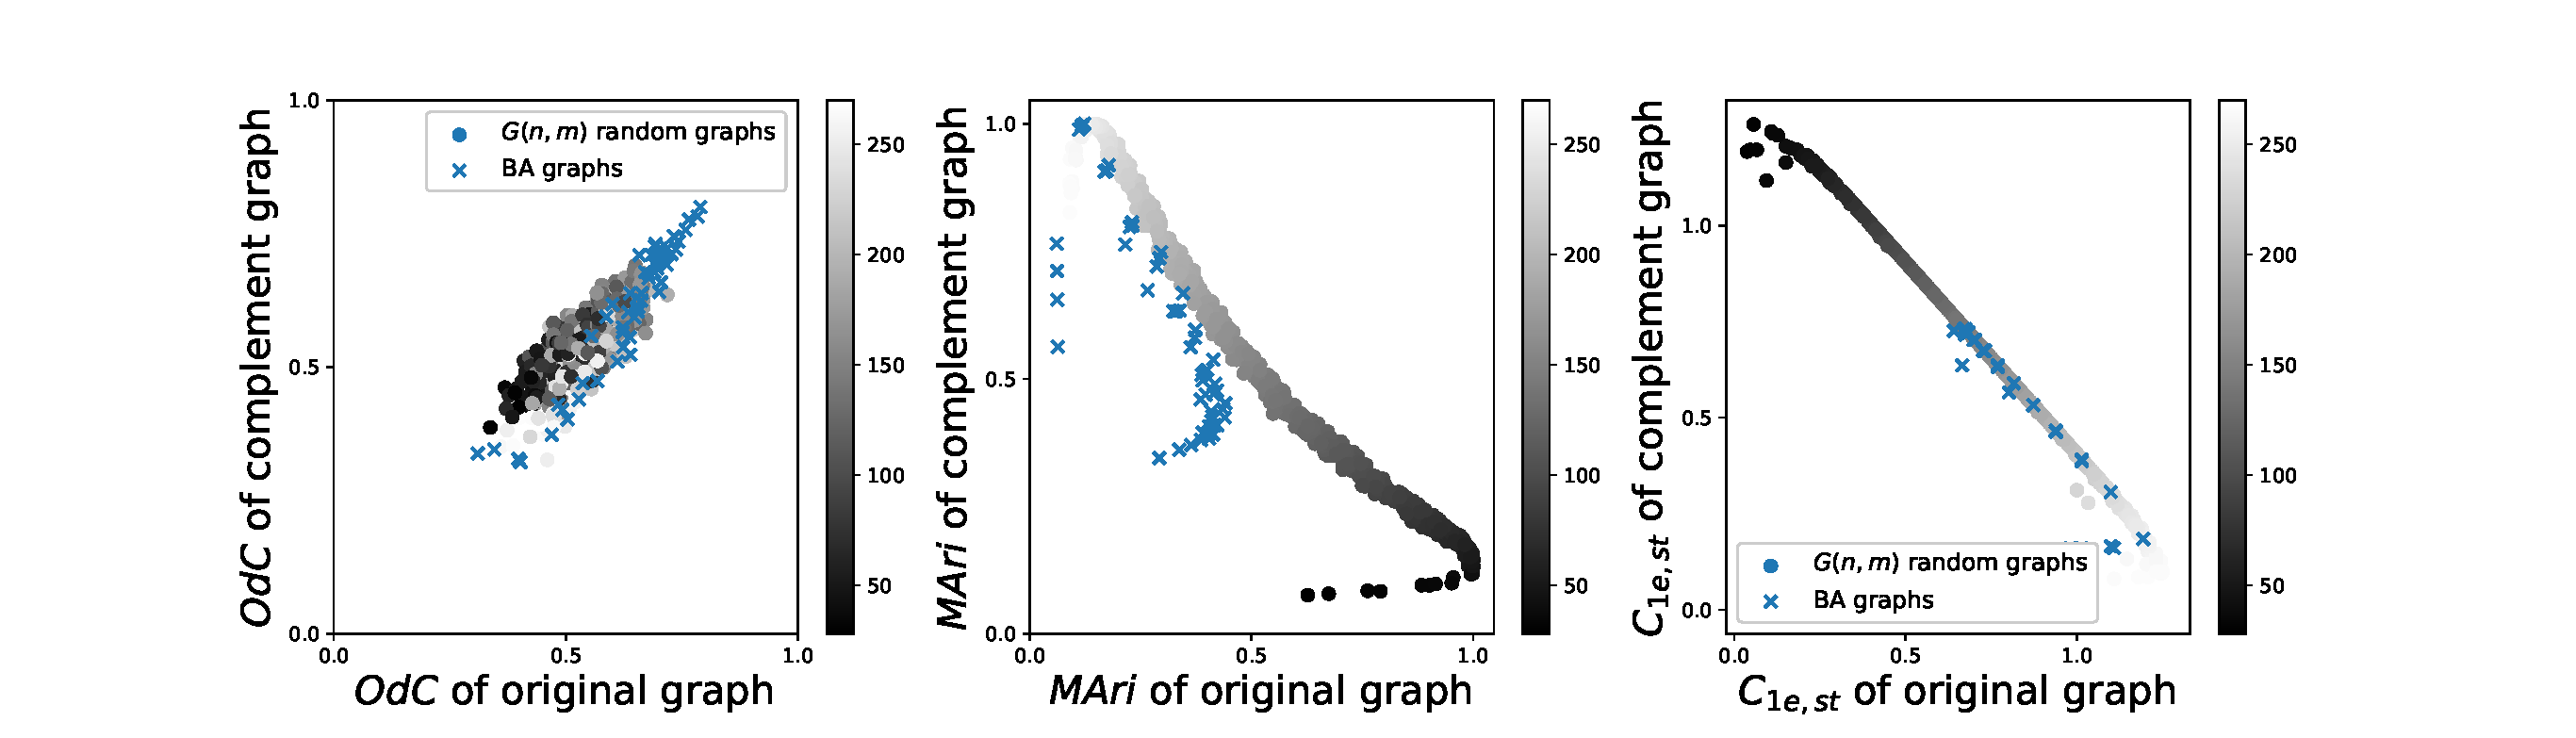
\includegraphics[width = \textwidth]{complement.eps}
    }
    \caption{Complexities of the original graphs and complement graphs with $n=20$. There are two types of graphs are generated: 500 $G(n,m)$ random graphs and 100 BA graphs.}
    \label{fig:complement}
\end{figure}
\noindent
$OdC$ seems to be very symmetric with respect to $m$. Since taking the completment graph is reversing the degree distribution, the consistency of node-node link relation is preserved. Causing the complexity value for original graph equal to the complement graph. As mentioned $MA_{RI}$ is highly based on the number of edges, so observing a linear function is not a surprise. This alo applies to BA grapps. Similar to $MA_{RI}$, $C1_{1e,st}$ is more keen to $m$, causing another negative correlation between the original graph and the complement graph.\\


\subsection{Applying $MA_{RI}$ on real networks}
To test the new measure $MA_{RI}$, 6 real networks are collected. To ensure comprehensive evaluation, various types of networks are used. To be applicable, bus networks in 6 cities are collected and converted to networks from raw. Bus networks are different to other real networks. Bus networks contain extraordinary amount of nodes with degree 2. For simplification and general interest, bus networks are modified. In modified bus networks, all nodes with $k=2$ are removed, whereas the edges are preserved. For instance, node $b$ is only conneted to $a$ and $c$. Node $b$ will be removed from the network and a new edge $(a,c)$ will be added to the network. The modification will be iterated multiple times until bus networks are free from node with degree $k=2$. Modification will significantly decrease the distance of bus networks. Moreover, generated graphs are also added to be evaluated and compared.\par
To be mentioned, we will refer these non-bus networks as real networks, for convinience.

\begin{table}[ht]
    \noindent\makebox[\textwidth]{
        \begin{tabular}{|c|c|c|c|c|c|c|c|c|}
            \hline
            Label & Name & Type & n & m& L & $L_r$ &$MA_{RI}$&$OdC$\\
            \hline
            \multicolumn{9}{|c|}{Real networks}\\
            \hline
            1 &  Dolphins\cite{dolphins} & Animal interaction & 62 & 159 & 3.357 & 2.524 & 0.999 & 0.517\\
            \hline
            2 &  PDZBase \cite{pdzbase}& Protein interaction & 161 &209 & 5.326 & 5.326 & 0.824 & 0.310\\
            \hline
            3&  Hamsterster\cite{hamster} & Online social network & 874 & 4003 & 3.217 & 3.058 & 0.963 & 0.532\\
            \hline
            4& Roget's Thesaurus \cite{roget}& Synonym network &994 & 3640 & 4.075 & 3.466 & 0.960 & 0.392\\
            \hline
            5 & Flight\cite{flight} & Flight network & 3397 & 19230 & 4.103 & 3.350& 0.948 & 0.525\\
            \hline
            6 & UK train \cite{GBPT}& UK train network & 2490 & 4377 & 10.384&6.220 & 0.664 & 0.233\\
            \hline
            \multicolumn{9}{|c|}{Bus networks}\\
            \hline
            7&\multicolumn{2}{c|}{London\cite{GBPT}}&8653&12285&32.338&8.687&0.38&0.127\\ 
            \hline
            8&\multicolumn{2}{c|}{Paris\cite{bus_collection}}&10644&12309&47.631&11.059&0.173&0.065\\ 
            \hline
            9&\multicolumn{2}{c|}{Berlin\cite{bus_collection}}&4316&5869&33.284&8.366&0.358&0.134\\ 
            \hline
            10&\multicolumn{2}{c|}{Sydney\cite{bus_collection}}&22659&26720&36.131&11.688&0.173&0.064\\ 
            \hline
            11&\multicolumn{2}{c|}{Detroit\cite{bus_collection}}&5683&5946&70.513&11.708&0.062&0.020\\ 
            \hline
            12&\multicolumn{2}{c|}{Beijing\cite{beijing}}&9249&14058&27.891&8.214&0.441&0.167\\ 
            \hline
            \multicolumn{9}{|c|}{Modified Bus}\\
            \hline
            13&\multicolumn{2}{c|}{London}&3417&6018&18.308&6.462&0.553&0.128\\ 
            \hline
            14&\multicolumn{2}{c|}{Paris}&2762&4301&15.386&6.975&0.468&0.106\\ 
            \hline
            15&\multicolumn{2}{c|}{Berlin}&1662&2941&18.36&5.867&0.586&0.149\\ 
            \hline
            16&\multicolumn{2}{c|}{Sydney}&4834&8358&17.665&6.838&0.49&0.089\\ 
            \hline
            17&\multicolumn{2}{c|}{Detroit}&295&483&6.341&4.794&0.643&0.117\\ 
            \hline
            18&\multicolumn{2}{c|}{Beijing}&4072&8325&14.864&5.902&0.64&0.195\\ 
            \hline
            \multicolumn{9}{|c|}{Generated networks}\\
            \hline
            19&\multicolumn{2}{c|}{G(n,m) random network($n=875,m=4000$)}&875&4000&3.313&3.061&0.970&0.330\\
            \hline
            20&\multicolumn{2}{c|}{WS network($n=875,k=10,p=0.05$)}&875&4375&5.000&2.942&0.974&0.123\\
            \hline
            21&\multicolumn{2}{c|}{NW network($n=875,k=10,p=0.05$)}&875&4587&5.075&2.883&0.980&0.089\\
            \hline
            22&\multicolumn{2}{c|}{BA random network($n=875,m=5$)}&875&4350&2.922&2.950&0.999&0.358\\
            \hline
        \end{tabular}
    }
    \caption{Label,description and parameters of used networks} 
    \label{tb:descriptions}
\end{table}


\begin{figure}[ht]
    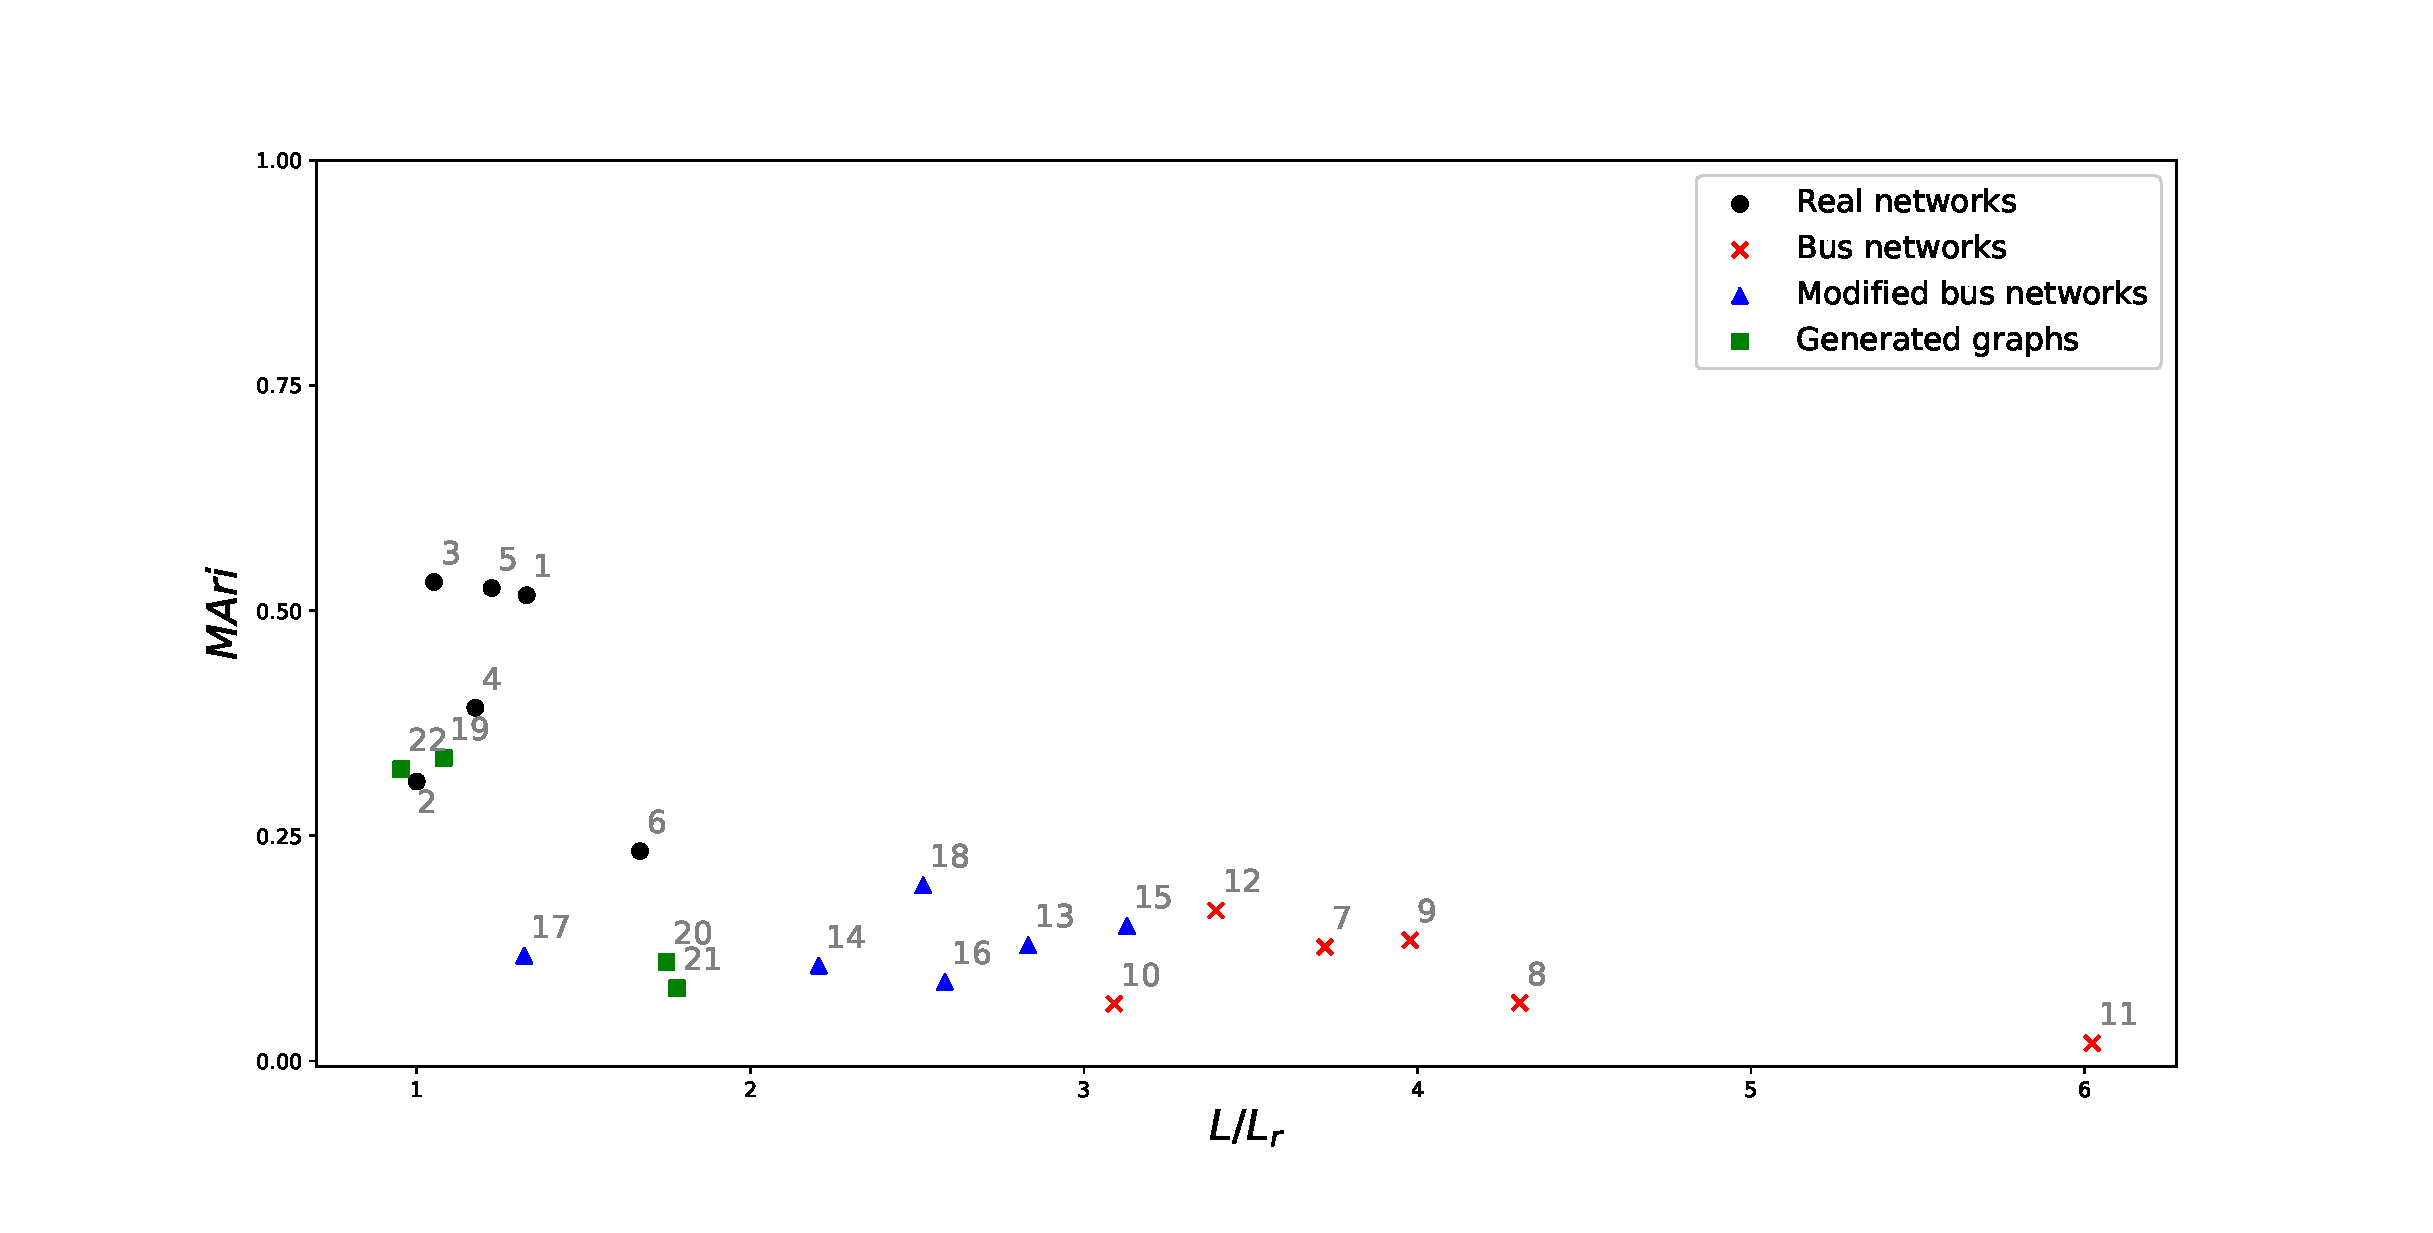
\includegraphics[width = \textwidth]{real_networks.eps}
    \caption{$MA_{RI}$ complexity of real networks, bus networks, modified bus networks and graphs generated by graph models, labelling and description can be found in table \ref{tb:descriptions}.}
    \label{fig:real_networks}
\end{figure}
\par
After careful consideration, average distance ratio $L/L_r$ is chosen to be the variable showin on x-axis in figure \ref{fig:real_networks}. Average distance is a more important parameter to consider about because it can identify how "small-world" the network is. As suggested, all the bus networks have significantly higher average distance ratio than real networks. Even after modified, the average distance ratios are still relatively high. But higher average distance ratio brings less $MA_{RI}$ complexity. We can suggest a negative correlation between the average distance ratio and the $MA_{RI}$ complexity. There is an exception of real networks, which is the UK train network. Cosidering the similarity between bus networks and train networks, it is not surprising. Generated graphs also behaves similar to standard real networks; low average distance ratio with high complexity, as they are intended to simulate the behaviour of standard real networks. In theory, "Flight" is also a public transport, so it should behave similar to bus networks or the train network. However, the "Flight" network performs unlike transport networks. Flight networks are designed to be robust\cite{zhixing2021recent} to be functional under severe whether/accident. Unlike trains or buses, flight are less limited by physical path in the sky.\par
To discuss the cause of increase of $MA_{RI}$ complexity after modified, we need to consider about the parameter $MA_{RI}$ focusing on. $\sum_{i,j>i}d_id_j$ is the only variable that affects the complexity of a graph. The essence of the measure is calculating the average $d_id_j$. By removing nodes with degree 2, average $d_id_j$ will be increased, and leads to an increase of the $MA_{RI}$ complexity.

\subsection{Rewiring on real networks}
As recommened in section \ref{rewiring}, rewiring is an important technique to monitor the behaviour of a network. Hence, we rewired real networks and modified bus networks to record their behaviour. Both single link rewiring and pairwise rewiring will be used. The reason we are going to use $OdC$ instead of $MA_{RI}$ is that pairwise rewiring will keep the degree relationship, and $MA_{RI}$ will stay unchanged.\par
How we rewire graphs:
\begin{itemize}
    \item The rewiring is done gradually. Initially, graph $G$ will be rewired with probability $p=0.05$. After recording the results, we rewire it with probability $p=0.05$ again. This step will be repeated 20 times.
    \item Both rewiring have been simulated on all graphs more than 10 times("dolphins" and "PDZBase" have been rewired more than 100 times, as they are relatively small), to generate more consistent results.
\end{itemize}
\begin{figure}[ht]
    \centering
    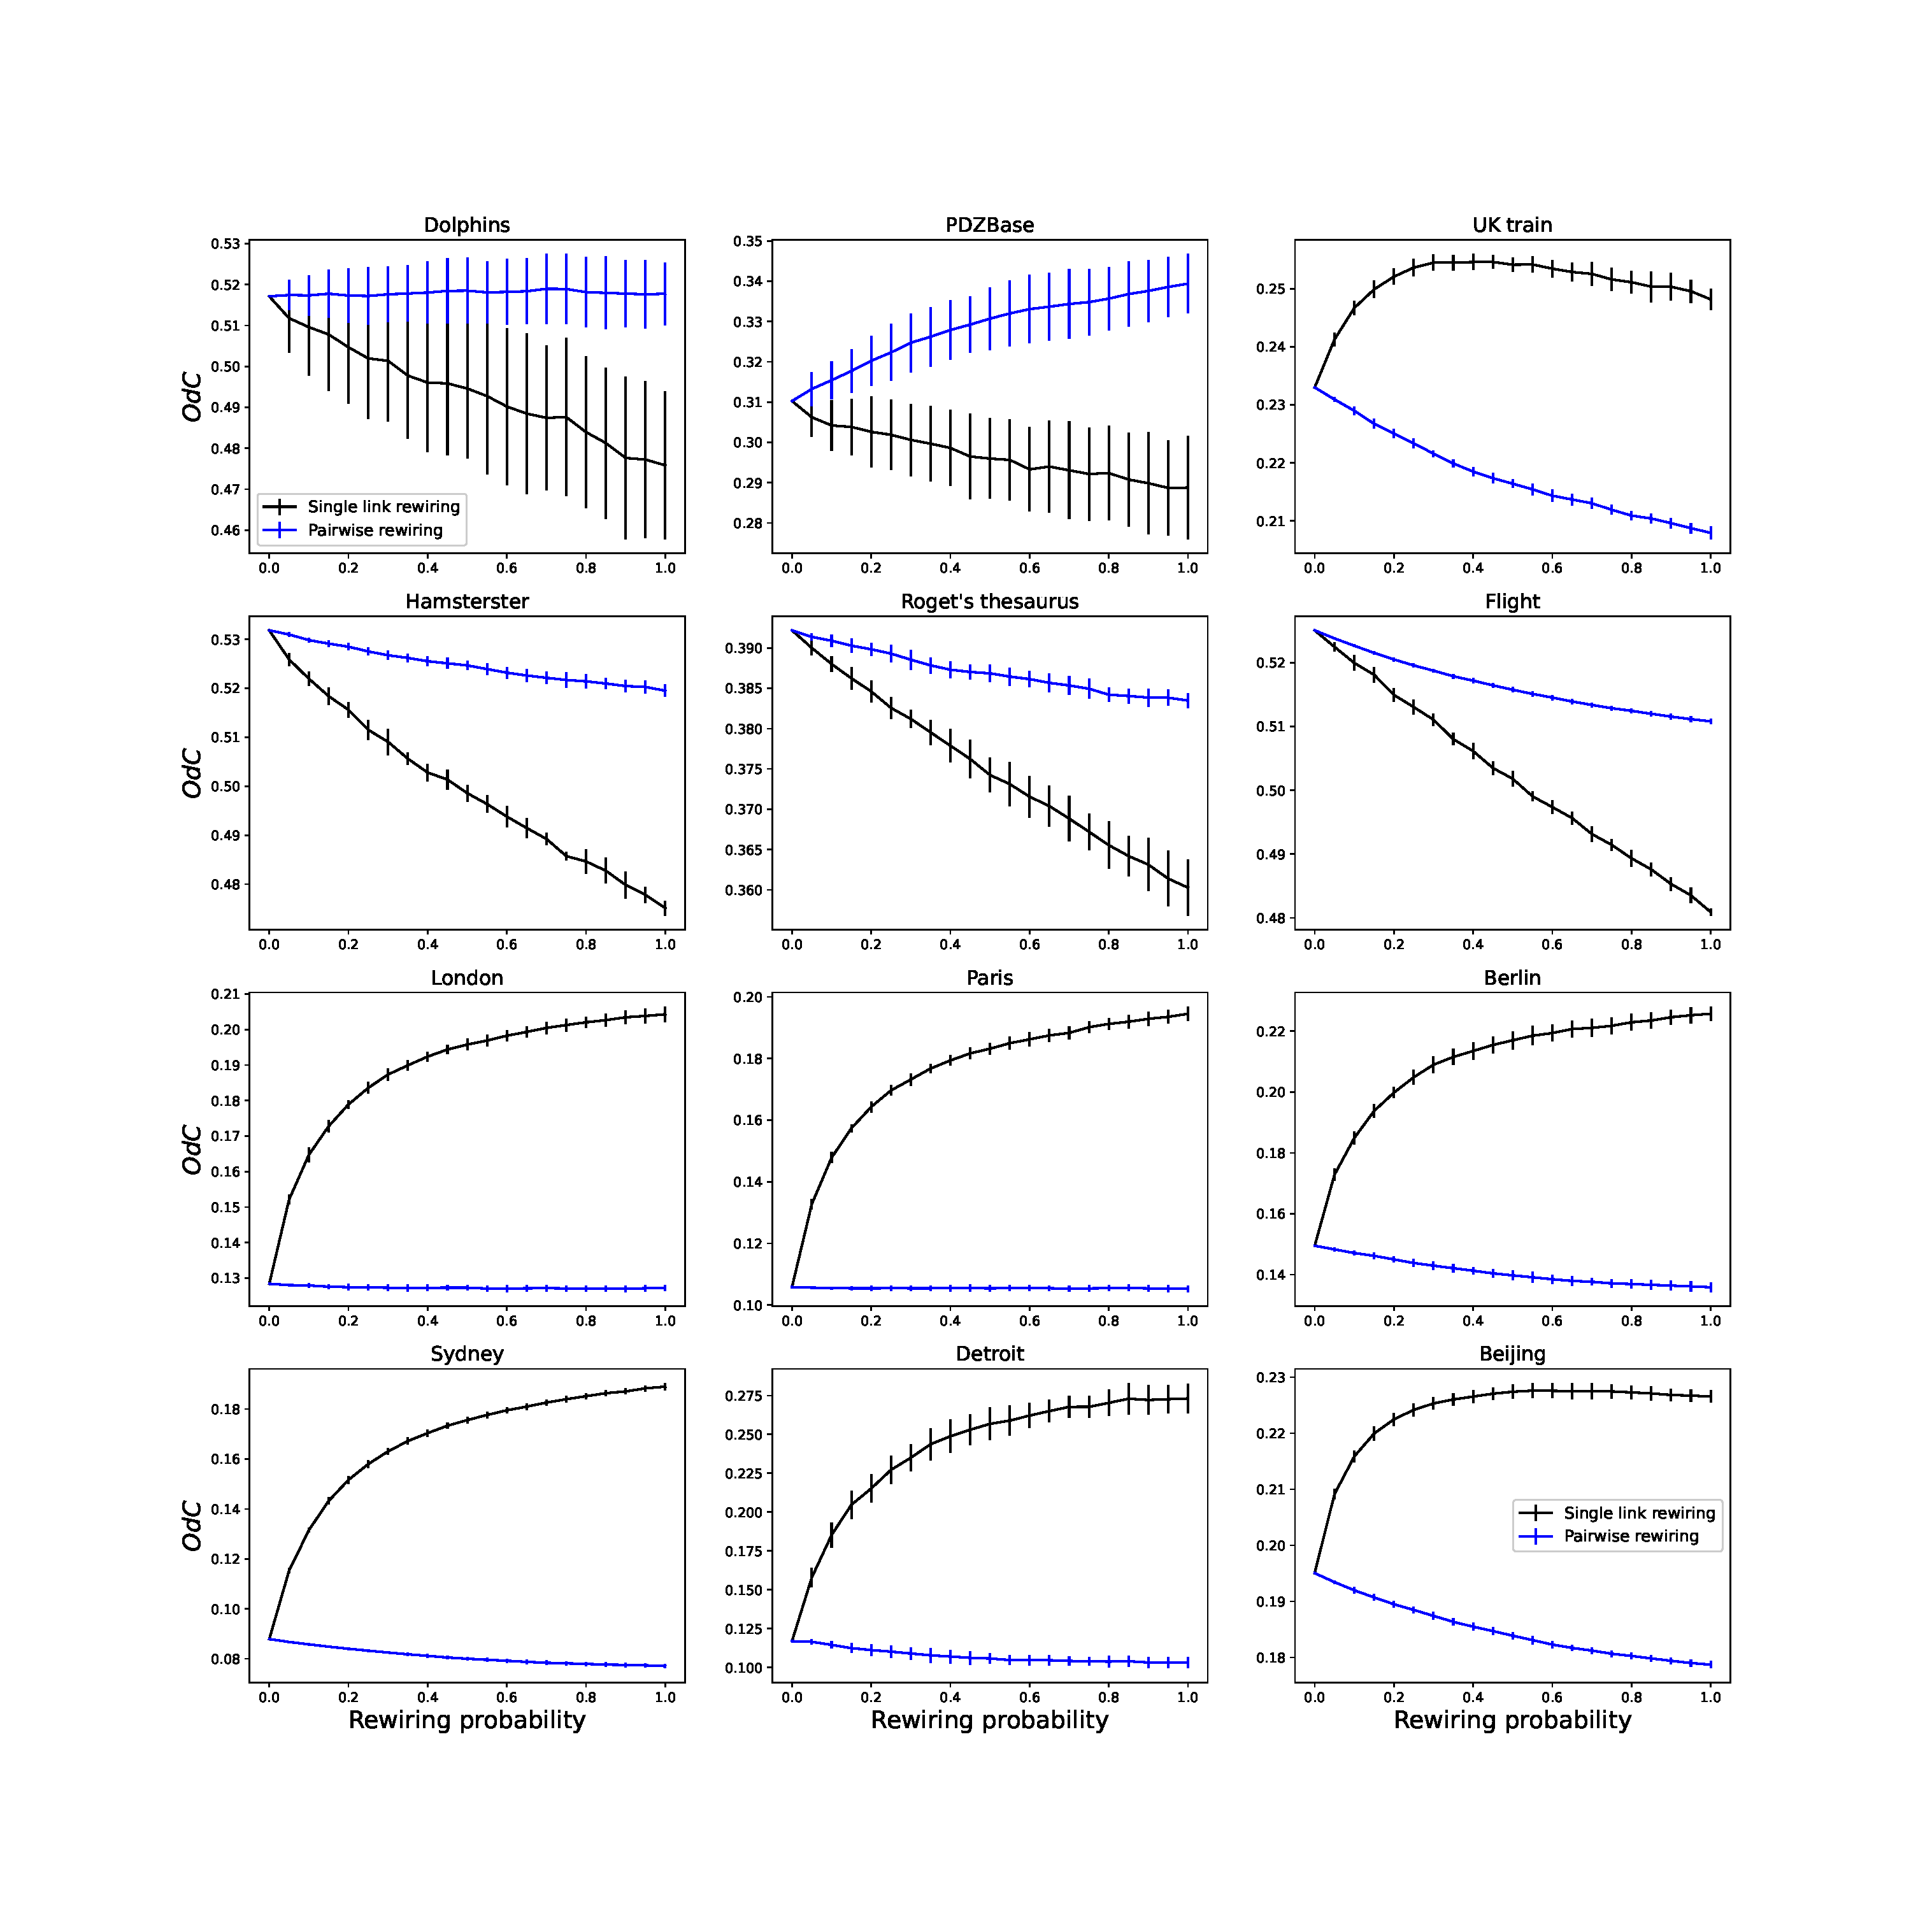
\includegraphics[width=\textwidth]{rewiring.eps}
    \caption{Change of $OdC$ complexities respect to change of rewiring probaility with an error bar(one standard deviation).}
    \label{fig:rewiring}
\end{figure}
\noindent
From figure \ref{fig:rewiring}, we can concludes that most real networks behaves similar using rewiring. As mentioned in section \ref{rewiring}, single link rewiring results in higher randomness, because it destroys the degree distribution. In theory, when $p=1$, the graph becomes a random network. $OdC$ decreases significantly with the increase of rewiring probability for real networks, whereas the change of complexity is not large for pairwise rewiring. This is because $OdC$ is highly sensitive to degree relationship, but pairwise rewiring does not change the degree relationship. Also, the error bar for "dolphins" and "PDZBase" is large. This is simply because they are small networks, rewiring will make larger impact than larger graphs.\par
There is an expcetion in real networks; the UK train network performs similar to bus networks rather than real networks. As public transportation networks, single link rewiring will cause the complexity to increase. Generally, the increase of complexity becomes small after $p=0.4$; almost half of the links have been rewired. As shown in table \ref{tb:descriptions}, $OdC$ complexities are very low for all the bus networks. As introduced by Claussen\cite{odc}, $OdC$ assign high complexity to graphs that have no preference for the degree of their neighbours. After destroying the degree correlation using single link rewiring, the $OdC$ complexity will increase.\par
In contrast, pairwise rewiring will cause the complexity to decrease briefly like real networks, with similar reason.
\section{Conclusion and further study}
In this theis, we investigated and compared difference of complexity measures. Different complexity measure focuses on different properties and parameters of a graph. For example, different subgraph measures focusing on the general structure of subgraphs, leads to high complexity and not feasible to apply difference subgraph measures on large networks. In addition, the floating point algorithmetic is imperfect when dealing with large numbers and decimals.
On the other hand, product measures are faily simple in terms of calculation time. Espectiall $Cr$, the easist complexity measure, which can be calculated in $O(n)$ time\cite{KIM20082637}. A drawback of product measures is that they are highly based on $m$, creating smaller difference than other complexity measures with fix $m$ and $n$.
$OdC$ measure can distinguish random graphs and graphs generated using BA,WS and NW model, and within relatively small amount of time. However, the complexity value are spreaded. We suggest to use the measure that is most suitable, depending on which specific parameters or properties are most important in the problem.\par
Additionally, we constructed a new measure $MA_{RI}$ based on the idea of $MA_g$. $MA_{RI}$ assigns higher complexity to sparser graph than $MA_g$. To be noticed, to calculate $MA_{RI}$, $R_{clique}$ and $I_{path}$ are not required, but $m$ is involved in the calcualtion.\par
We also compare the difference between real networks and bus networks, and we investigated the unique property of bus networks: high average distance with low complexity, which is the opposite of a small-world network. This causes averagely lower complexities than other real networks.\par
There are more complexity measures \cite{emmert-streib_dehmer_2012}\cite{dehmer_barbarini_varmuza_graber_2009} for further studies and researches. We encourage study and application of the measures on different type of graphs and monitor the behaviour of different complexity measures. Further studies on complexity measures could help the network science community to build a comprehensive, robust and applicable complexity meausre which everyone can agree on.\par
An unexpected fact was observed: degree based measures($OdC$,$MA_g$,$MA_{RI}$) generally assign relatively high complexity to very sparse graphs, except $Ce$. We are not sure whether this is a coincidence or not, but this can be a topic to further investigate.\par
Overall, we hope our result can stimulate more studies on network complexity meausre. The definition of complexity is already difficult to be determined. A good complexity measure should be able to distinguish: random networks, small-world networks, scale-free networks and real networks. In addition, highest complexity to graphs with number of edges slightly less than the medium. Our work provides useful aspect and observation to build a optimal complexity measure in the future.


\end{document}